\input{../preamble.tex}
% \bibliographystyle{plain} % Style BST file (bmc-mathphys, vancouver, spbasic).
% \bibliographystyle{unsrt} % Style BST file (bmc-mathphys, vancouver, spbasic).
% \bibliography{pubs.bib}      % Bibliography 
\bibliography{pubs.bib}
\title{Projekt 4 - rapport}
\author{Team 2}
\newcommand{\myparagraph}[1]{\paragraph{#1}\mbox{}\\}
\begin{document}

\lstset{language=C,%
  % basicstyle=\color{red},
  breaklines=true,%
  morekeywords={matlab2tikz},
  keywordstyle=\color{blue},%
  morekeywords=[2]{1}, keywordstyle=[2]{\color{black}},
  identifierstyle=\color{black},%
  stringstyle=\color{mylilas},
  commentstyle=\color{mygreen},%
  showstringspaces=false,%without this there will be a symbol in the places where there is a space
  % numbers=left,%
  % numberstyle={\tiny \color{black}},% size of the numbers
  % numbersep=9pt, % this defines how far the numbers are from the text
  emph=[1]{for,end,break},emphstyle=[1]\color{red}, %some words to emphasise
  % emph=[2]{word1,word2}, emphstyle=[2]{style},    
}


\maketitle
\thispagestyle{empty}

\textbf{Deltagere:}
\begin{figure}[h]
  \centering
  % BEGIN RECEIVE ORGTBL delt
  \begin{tabular}{|p{5cm}p{10cm}|}
    \hline
    &\\
    Stud. nr: 201602094 & Navn: Søren Holm Korsgaard \\
    \hline
    &\\
    Stud.nr.: 201607563 & Navn: Jacob Gustafsson \\
    \hline
    &\\
    % Stud.nr.: 201704859 & Navn: Jonas Buus \\
    % \hline
    % &\\
    Stud.nr.: 20084327 & Navn: Simon Rasmussen \\
    \hline
    &\\
    Stud.nr.: 201704483 & Navn: Thomas Dueholm Jensen \\
    \hline
  \end{tabular}
  % END RECEIVE ORGTBL delt

\end{figure}
\vspace{-5mm}
% \clearpage
\setcounter{tocdepth}{3}
\setcounter{secnumdepth}{4}
\clearpage
\tableofcontents
\thispagestyle{empty}
\newpage
% \pagenumbering{arabic}
\setcounter{page}{1}

% \section{Introduktion}
% \label{sec:introduktion}

\section{Introduktion (Jacob)}
\label{sec:introduktion-1}

Denne projektrapport sammenfatter vores arbejde, igennem PRO3 og PRO4, med at bygge en Hybrid Drone Power Pack - herefter benævnt HDPP.

Projektet har været at bygge et system, som kan kobles på en drone for at forlænge flyvetiden. Problemstillingen består i, at de fleste moderne droner, har en meget kort flyveradius, da batterierne er meget tunge i forhold til energikapacitet. Den begrænsede flyvetid gør dronerne uegnede til opgaver som pakkelevering, flyvning med blodprøver og andet leveringsarbejde, som man ellers har spået, kunne automatiseres med dronerne.

Da energitætheden i benzin er væsentlig højere, end i et lithiumbatteri, bygges en HDPP der baseres med en brændselsmotor med tilhørende generator. På denne måde har vi mulighed for at lade batterierne mens vi flyver. 

Nedenfor følger de krav, som er sat op af kunden, henholdsvis de krav som vi har specificeret for det færdige produkt.

\subsection{Kundens (undervisers) krav}
\label{sec:kravsspecifikation-1}

\subsubsection{Funktionelle}
\label{sec:funktionelle}

\begin{itemize}
\item Udgangsspændingen fra HDPP skal være kompatibel med spændingen på standardbatteripakken
\item HDPP skal startes enten elektrisk eller mekanisk med håndkraft 
\item Kapaciteten på HDPP’en skal være tilstrækkelig til at lande dronen sikkert, hvis forbrændingsmotoren svigter.
\item HPP’en skal besidde en basal logning, så man kan udlæse performance.
\end{itemize}

\subsubsection{Designspecifikke }
\label{sec:designspecifikke-}

\begin{itemize}
\item Komponenter skal udvælges så de på bedste vis er et kompromis mellem lav vægt, pris og performance.
\item Brug så vidt muligt tilgængelige mekaniske dele - herunder forbrændingsmotor. 
\item En microcontroller skal sikre kontrol over systemet.
\end{itemize}

\subsection{Preprojekt}
\label{sec:preprojekt-}

For at synliggøre produktets formåen og berettigelse, har vi valgt at gengive vores storytelling og Rich Picture fra vore preprojekt. Begge har de til formål at give et meget generelt og råt overblik over systemet, på et niveau som alle kan forstå.

\subsubsection{Storytelling}
\label{sec:storytelling-}

Endelig er det lørdag! Du vågner alt for tidligt i bare spænding, for endelig er det lørdag, og du skal ud og flyve med drone. Dronecertifikatet er endelig i hus, og din store DJI S1000 drone er klar. Med batteriet på 100\%, smider du det hele i bilen og kører mod stranden. Der skal tages billeder af morgensolen fra helt nye vinkler. Med det påmonterede kamera, er det ingen sag.

Du ankommer til stranden, kaffen er drukket og du kan mærke hjerterytmen stige - nu skal det være. Du får, let og elegant, dronen i luften og taget nogle gode billeder. Pludselig, og uden varsel, vender dronen tilbage til dig. Du undrer dig meget, og først idet den lander foran dig, kommer du i tanke om den, mildest talt, elendige flyvetid dronen har på batteripakken. Kun omkring 15 minutter! Som du står der og ærgre dig, går de sidste skyer fra solen, og du kunne have fået de perfekte billeder du drømte om. 
Ovenstående scenarie har vi sat os for at undgå. Dette gøres ved at etablere en forbrændingsmotor og koble til dronens batterisystem gennem en generator. På denne måde lader dronen mens du flyver, og flyvetiden bliver forlænget markant!

\subsubsection{Rich Picture}
\label{sec:rich-picture-}

Herunder ses vores Rich Picture, som en konstrueret lige efter opgaven er blevet stillet.

\begin{figure}[h]
  \centering
  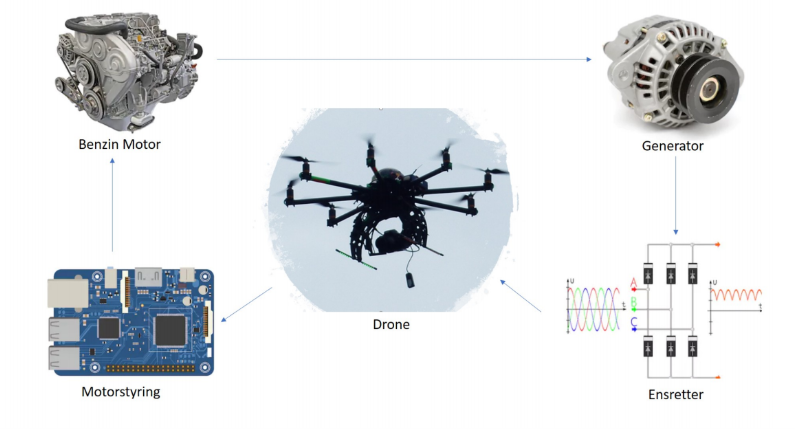
\includegraphics[width=0.8\textwidth]{int1.png}
  \caption{Rich Picture}
  \label{fig:int1}
\end{figure}

\subsubsection{Kravspecifikation}
\label{sec:kravspecifikation}

På baggrund af ovenstående begyndte vi at opstille specifikke, tekniske krav til produktet - blandt andet på baggrund af de af underviserne stillede krav,. I en kravsanalyse specificeres de krav, der er til det færdige produkt eller produktets enkelte komponenter.En udbytterig kravsanalyse indebærer at kunden inddrages.Kravene er nedenfor opstillet efter EARS-princippet (EARS:Easy to Approach Requirements Syntax).

Kravene er inddelt udfra ufravigelige (ubiquitous), begivenhedsorienterede (event-driven), driftsorienterede(state-driven) og fejlorienterede krav (unwanted behaviour). EARS-princippet muliggør således en prioritering af kravene.

\myparagraph{Ubiquitous}
\label{sec:kravspecifikation-1}

\begin{enumerate}
\item Motoren skal kunne startes vha. BLDC-generator.
\item Udstødning skal monteres sådan at varmen ikke påvirker dronen.
\item Generatoren skal levere en middeleffekt på 2450 W ved 22,2 V (110,3 A)
\item Generatoren skal være 3-faset jf. projektbeskrivelsen.
\item HPP må maksimalt veje 5 kg.
\item Ensretteren skal kunne klare at håndtere en effekt af 2,45 kW.
\item Ensretteren skal modtage 3-faset vekselstrøm og levere en jævnstrøm.
\item HPP skal inddæmmes, så den kan modstå vejrforhold, jf. IP56 standard.
\item Ensretteren må maksimalt have ripple på 1V output.
\end{enumerate}

\myparagraph{Event Driven}
\label{sec:kravspecifikation-2}

\begin{enumerate}
\item I tilfælde af nødlanding skal motoren deaktivere. 
\end{enumerate}

\myparagraph{State Driven}
\label{sec:kravspecifikation-3}

\begin{enumerate}
\item HPP skal fungere korrekt før dronecopterens motorer igangsættes ved take-off.
\item Når motoren er aktiv, skal omdrejninger reguleres efter belastning af ladestrømmen.
\item Når generatoren ikke er i fulde omdrejninger, skal dronen ikke kunne lette.
\item Der skal defineres et effekt setpunkt til kontrol af opstart.
\item Når generatoren genererer strøm, skal input og output til/fra ensretteren overvåges og logges.
\end{enumerate}

\myparagraph{Unwanted}
\label{sec:kravspecifikation-4}

\begin{enumerate}
\item Dronecopterens motorer vil tillade nødlanding ved fejl i moteren.
\item Hvis der opstår fejl i motoren, vil dronen lande når spændingen falder på batteriet.
\item Hvis generatoren ikke opnår fulde omdrejninger inden 10 sek. efter motorstart, afbrydes motoren.
\item Hvis udgangsstrømmen ikke når setpunktet (PID-regulering), skal dronen nødlande.
\end{enumerate}

\subsubsection{Blokdiagram}
\label{sec:blokdiagram-}

På baggrund af alt det ovenstående, samt flere andre overvejelser, som der kan læses mere om i den vedlagte preprojekt rapport, endte vi op med følgende blokdiagram over de forskellige subsystemer.

\begin{figure}[h]
  \centering
  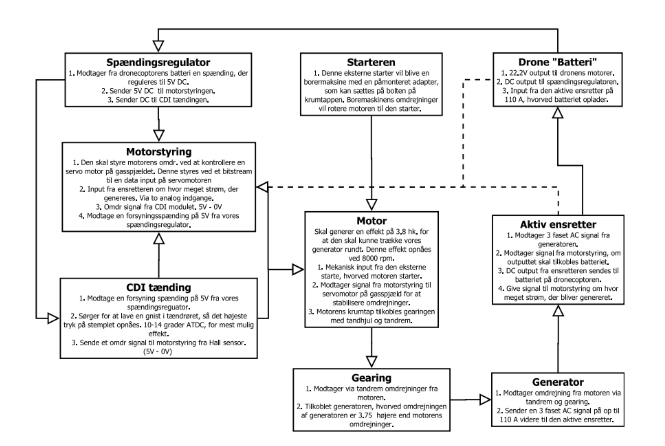
\includegraphics[width=0.8\textwidth]{int2.png}
  \caption{Blokdiagram}
  \label{fig:int2}
\end{figure}
% \subsection{Hypotese}
% \label{sec:hypotese}


\clearpage
\section{Baggrund}
\label{sec:baggrund}

\subsection{Aktive ensretter (Søren og Thomas)}
\label{sec:aktive-ensretter}

Ét af HPP’s primære subsystemer er blokken, der skal stå for ensretningen af den tre-fasede strøm/spænding, der genereres fra forbrændingsmotoren og generatoren. Der har i processen været mange essentielle dilemmaer og prioriteter, der skulle afklares for at få den mest optimale løsning. Da der foreligger et grundlæggende ønske om at holde den samlede vægt på HPP nede på et acceptabelt niveau, var det nærliggende at forsøge at realisere ensretningen aktivt. Hvad dette vil sige, berøres i det efterfølgende afsnit.

\subsubsection{Passiv vs. aktiv ensretning}
\label{sec:passiv-vs.-aktiv}

I en typisk ensretter (en passiv ensretter) anvendes en diodekonstruktion, som tillader et AC-signals positive cyklus at passere til outputtet, for derefter at invertere den negative del af cyklussen. Resultatet er et udelukkende positivt signal, med en variabel spændingsamplitude. Da vi forventer at lede ca. 110 A gennem systemet, er dioder ikke anvendelige. Spændingsfaldet over dioder ligger typisk i omegnen af 0.3-0.7V, og det vil betyde et effektab, som motoren skal kompensere for via flere omdrejninger.

I stedet anvendes en “Ideal Diode Controller”, som har til formål at levere spænding til gate-terminalen på MOSFET transistorer. En MOSFET har i cut-off tilstand en diodelignende opførsel, men når de leder optimalt, er modstanden i transistoren meget lav (helt ned til få m$\Omega$). Parallelkobles transistorer kan modstand sænkes yderligere. IC’en styrer, hvornår transistorerne åbner og lukker, og kontrollerer dermed AC-signalets passage gennem ensretteren, så output-signalet er positivt, ligesom ved en almindelig diode-ensretter. Denne styring gør, at ensretteren defineres som en aktiv ensretter.

\begin{figure}[h]
  \centering
  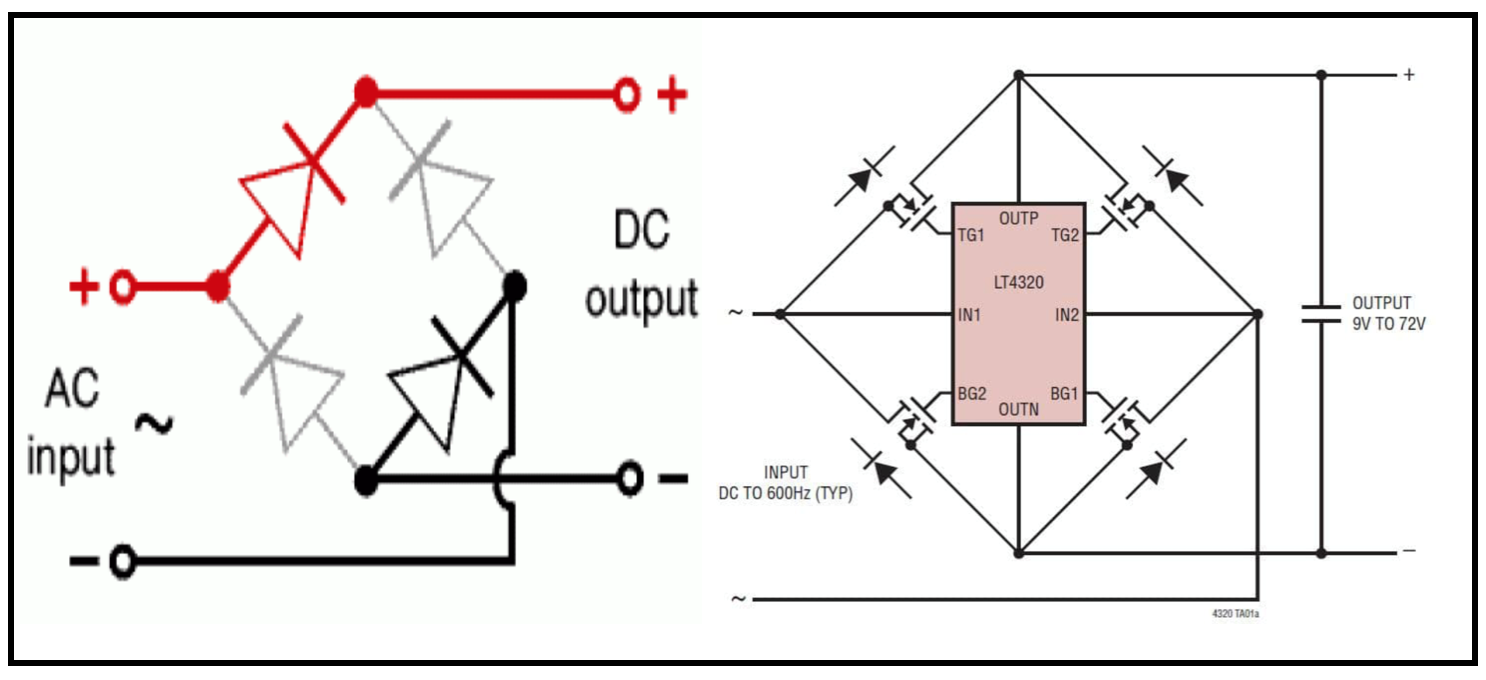
\includegraphics[width=0.8\textwidth]{prens1.png}
  \caption{Passiv vs. aktiv ensretning}
  \label{fig:prens1}
\end{figure}

Den store fordel ved aktiv ensretning kontra passiv er reduceringen af effekttabet gennem kredsløbet. Denne reduktion påvirker direkte, at forbrændingsmotoren skal køre med mindre RPM for at producere behovet til dronen, end hvis ensretningen var passiv. Derudover vil dimensioneringen af heatzinks til kredsløbet ligeledes være væsentlig mindre, da mindre effekttab betyder mindre varmeafledning.  
  
En generel udfordringen ved AC/DC konvertering er \textit{ripples} på output signalet. Ensrettes en enkelt AC-fase, får man et udgangssignal, med stor variation i spænding leveret. Kombineres tre faser med en faseforskydning på 120$^\circ$ mellem sig, som i vores tilfælde, vil summationen af de 3 sinuskurver generere et output signal med mindre \textit{ripple}.

\begin{figure}[h]
  \centering
  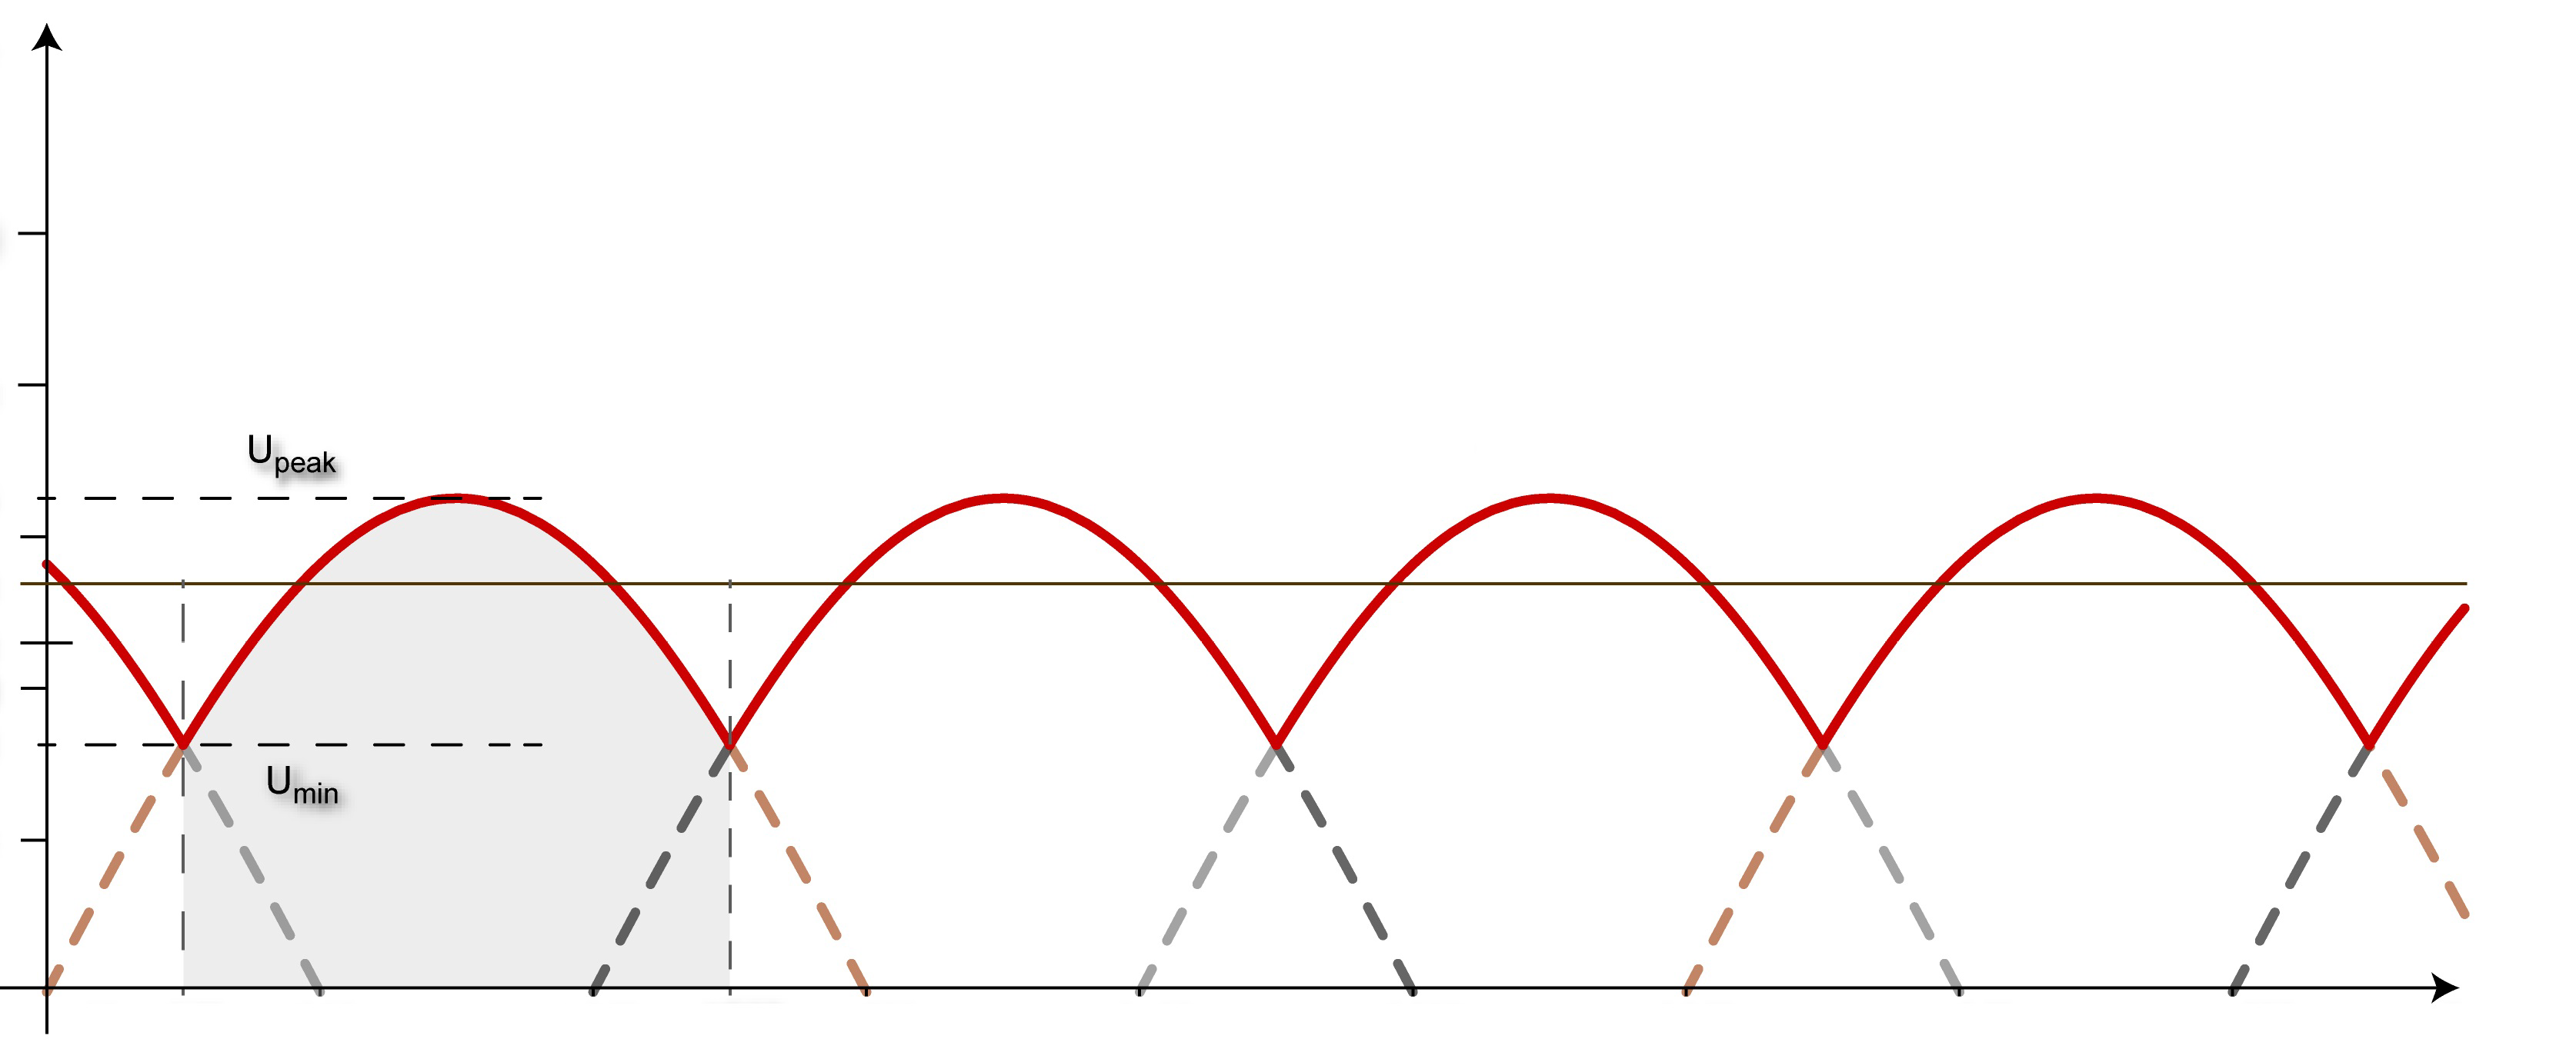
\includegraphics[width=0.8\textwidth]{prens2.png}
  \caption{Graf over ripple spænding på output signal som funktion af tid. Stiplet linje = ensrettet enkeltfase
AC-signal. Rød linje = ripple på kredsløb med kondensator parallelt på load. Kilde: Wikimedia Commons}
  \label{fig:prens2}
\end{figure}

Der vil stadig være \textit{ripple} til stede i signalet, og denne udjævnes til et acceptabelt niveau (for batteriet på drone) vha. kondensatorer. Kondensatoren lader, når $\frac{\mathrm{d}v}{\mathrm{d}t}$ på udgangssignalet er positivt og aflader, når spændingen igen falder. Den strøm kondensatoren afgiver adderes udgangssignalet, hvorfor $\frac{\mathrm{d}v}{\mathrm{d}t}$ øges.

\subsubsection{Valg af IC }
\label{sec:valg-af-ic}

I timebox 2 analyserede vi os frem til følgende valg af IC til realiseringen af kredsløbet til den aktive ensretter:
\begin{itemize}
\item Linear Technology, LT4320-1, Ideal Diode Bridge Controller
\end{itemize}

Dette skyldes bl.a., at den er designet specifikt til luftbårne strømforsyningssystemer, som kan håndtere frekvenser op til 600 Hz, 9-72V, og opfylder tidligere defineret krav om optimal effektivitet, og minimalt effekttab.

\begin{figure}[htb]
  \begin{minipage}{\textwidth}
    \centering
    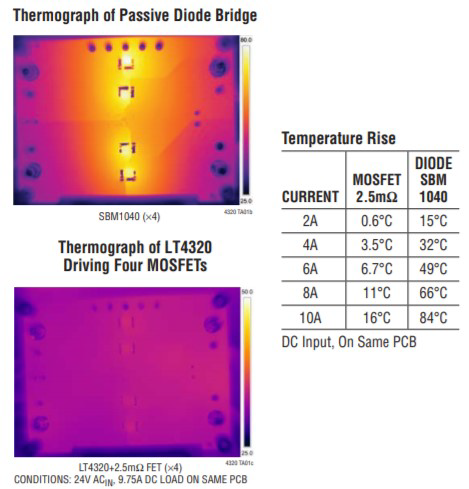
\includegraphics[width=0.8\textwidth]{prens3.png}
    \caption{Varmeudvikling. Passiv vs. LT4320\protect\footnotemark}
    \label{fig:prens3}
    \footnotetext{Fra databladet til LT4320-1. \url{https://www.analog.com/media/en/technical-documentation/data-sheets/4320fb.pdf}}
  \end{minipage}
\end{figure}

\subsubsection{Kredsløbet}
\label{sec:kredslobet}

Leverandøren af LT-4320-1, foreslår kredsløbet\footnote{url{https://www.analog.com/en/products/lt4320.html}} set på figur, som en yderst energieffektiv tre-faset aktiv ensretter.

\begin{figure}[h]
  \centering
  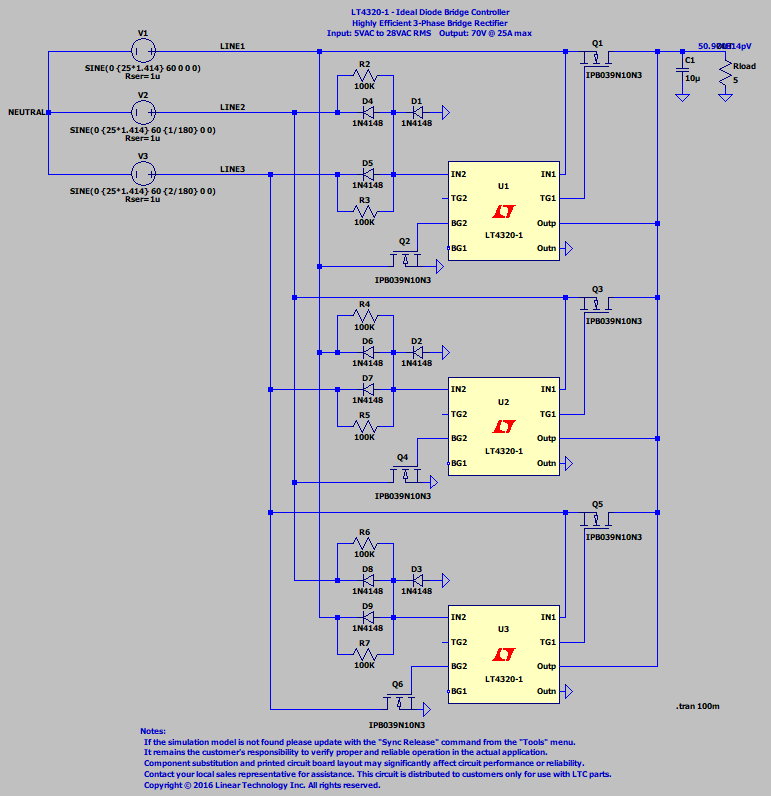
\includegraphics[width=0.8\textwidth]{prens4.png}
  \caption{Kredsløb til realiseringen af ensretteren}
  \label{fig:prens2}
\end{figure}

Vi valgte at arbejde videre med den opstilling. De næste afsnit indeholder en opsummering af simulering, realiseringen og test af kredsløbet.

\subsection{Spændingsregulator (Jacob)}
\label{sec:spandingsforstarker}



\subsection{Motorstyring (Simon)}
\label{sec:motorstyring}


Motorstyringen for systemet vil bestå i præcis justering af forbrændingsmotorens omdrejninger i forhold til dronecopterens strømforbrug. Det valgtes at arbejde med et simplere system for at fokuserer på principperne i motorstyring. Det betød at motorstyringen skulle bestå i udvikling af PID-regulering af forbrændingsmotoren sådan at der skulle foregå korrektion af motorens spjældvinkel i forhold til motorens omdrejninger.

Fjare\autocite{pid1} er en artikel der beskriver PID regulering af en forbrændingsmotor som skal drive en aerocopter. Der er taget inspiration fra denne tilgang inklusiv PID-regulering og PID-koefficienter.
% Målet med dette afsnit er at opstille en kravsspecifikation for motorstyringen samt at færdiggøre analysen af motorstyringen og lægge op til hvordan en test af motorstyring kan udformes for at præcisere PID-algoritme samt at opfylde krav.

% \lstdefinestyle{customc}{
%   belowcaptionskip=1\baselineskip,
%   breaklines=true,
%   frame=L,
%   xleftmargin=\parindent,
%   language=C,
%   showstringspaces=false,
%   basicstyle=\footnotesize\ttfamily,
%   keywordstyle=\bfseries\color{green!40!black},
%   commentstyle=\itshape\color{purple!40!black},
%   identifierstyle=\color{blue},
%   stringstyle=\color{orange},
% }

% \lstdefinestyle{customasm}{
%   belowcaptionskip=1\baselineskip,
%   frame=L,
%   xleftmargin=\parindent,
%   language=[x86masm]Assembler,
%   basicstyle=\footnotesize\ttfamily,
%   commentstyle=\itshape\color{purple!40!black},
% }

% \lstset{escapechar=@,style=customc}

\subsubsection{Kravsspecifikation}
\label{sec:kravsspecifikation}
Med baggrund i Fjare\autocite{pid1} sættes følgende krav:
\begin{itemize}
\item Overshoot skal ikke være mere en 197 rpm.
\item Justeringstiden må max være 8,8 sekunder.
\item Ifm. et step respons skal 90 \% af målet være opnået i mindre end 3 sekunder.
\item Det skal være muligt at vedligeholde en konstant hastighed over længere tid (dvs. mere end 5 minutter).
\item Servomotoren skal kunne reguleres.
\item Motoren skal kunne startes.
\item Omdrejningerne skal kunne måles.
\end{itemize}

\subsubsection{PID regulering}
\label{sec:overordnet-mal}

PID-regulering består i regulering af et output på baggrund af forskellen mellem det tilstræbte og det faktiske - dette kan kaldes fejlen. PID regulering kan beskrives med
\begin{equation}
  \label{eq:1}
  u(t)=k_Pe(t)+k_I \int_0^t e(\tau)\mathrm{d}\tau + k_D\frac{\mathrm{d}e(t)}{\mathrm{d}t}
\end{equation}

hvor $e(t)$ er fejl som funktion af tiden, $e(\tau)$ er fejl som funktion af den akkumulerede tid og $k_P$, $k_I$ og $k_D$ er koefficienter svarende til henholdsvis det proportionale, integrede og deriverede forhold. Det proportionale vil sige forholdet mellem tilstræbte og det faktiske for et givent tidspunkt. Det integrede vil sige forskellen mellem tilstræbte og det faktiske akkummuleret over tid. Det betyder at den integrerede koefficient viser en trend for fejlen. Det deriverede er et mål for hvor hurtigt fejlen ændrer sig over tid.

Formålet ved udarbejdelse af PID-regulering er at finde de optimale værdier af $k_P$, $k_i$ og $k_d$.

% For et givent sæt af K-værdier, udvælges en række forskellige typer af trinvise ændringer i hastigheden. Der måles på hvor lang tid det tager for ændringen at indfinde sig, samt hvor store udsving dette gør sig ud i.

Som udgangspunkt er det tidligere vist(\autocite{pid1}) at $K_p=0,065$ og $K_i=0,000005$ har været optimale, samt at $K_d$ helt blev droppet eftersom det ikke var en gavnlig parameter.

\subsubsection{Software}
\label{sec:software}

Fra Fjare\autocite{pid1} kunne et eksempel på et program være skrevet i pseudo C-kode:
\begin{lstlisting}[language=C,basicstyle=\ttfamily]
  void velPID ( ) {
    lowpassSpeed = alpha * lastLowpassSpeed + (1-alpha) * measuredSpeed;
    K1 = kp * setpointWeight * (setpointSpeed - lastSetpointSpeed) + kp * (lastMeasuredSpeed - lowpassSpeed);
    K2 = ki * (setpointSpeed - lowpassSpeed);
    K3 = kd * (2 * lastMeasuredSpeed - lowpassSpeed - lastLastMeasuredSpeed);
    output = lastOutput - K1 - K2 - K3;
    throttlePos = floor(output + 0.5);
    if(throttlePos<throttleopen){
      output = (double) throttleopen;
      throttlePos=throttleopen;
    }
    if(throttlePos>throttlesafe){
      output = ( double )throttlesafe;
      throttlePos=throttlesafe;
    }
    lastLowpassSpeed = lowpassSpeed;
    lastLastMeasuredSpeed = lastMeasuredSpeed;
    lastMeasuredSpeed = lowpassSpeed;
    lastSetpointSpeed = setpointSpeed;
    lastOutput = output;
    throttle.writeMicroseconds(throttlePos);
  }
\end{lstlisting}

\clearpage
\section{Metode og analyser}
\label{sec:metode}

\subsection{Aktive ensretter (Søren og Thomas)}
\label{sec:aktive-ensr-soren}

\subsubsection{Test af generators output spænding}
\label{sec:test-af-generators}

Inden vi anskaffede os IC’erne til kredsløbet, skulle det sikres, at forbrændingsmotor og generator i tomgangsdrift som minimum producerede 9 V (peak). Dette var nødvendigt for, at IC’erne var funktionsdygtige. \textcolor{red}{Der opstilles som følge af ovenstående konstatering et krav til den aktive ensretter.}\\

\begin{tabular}{p{1cm}l}
  \textcolor{red}{2.1.3.9}&\textcolor{red}{Der skal som minimum være 9 Volt (peak) på udgangen af generatoren, inden denne tilkobles}\\
  & \textcolor{red}{den aktive ensretter}\\
\end{tabular}

For at verificere dette blev der konstrueret et testsetup, hvor det var muligt at måle output spændingen på én af generatorens tre faser. Et blokdiagram over testsetuppet kan ses i nedenstående figur.

\begin{figure}[h]
  \centering
  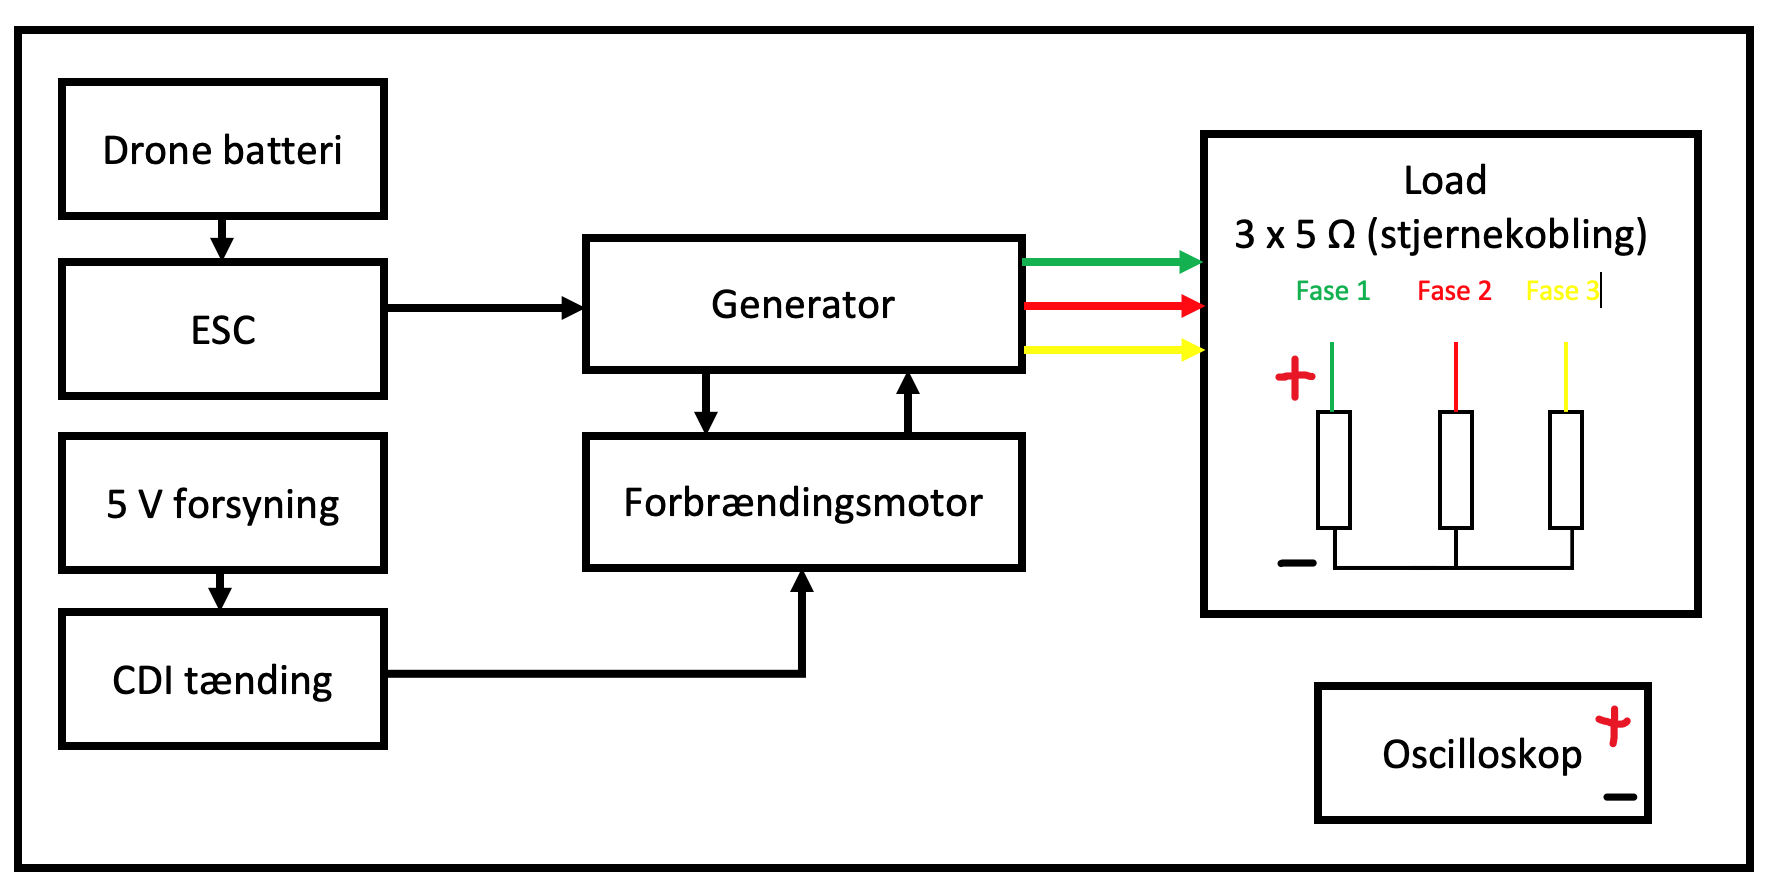
\includegraphics[width=0.8\textwidth]{prens5.png}
  \caption{Blokdiagram til test af outout spænding på en fase af generator}
  \label{fig:prens5}
\end{figure}

Testen viste, at der var en spænding på 11.4 V (peak)\footnote{Se bilag, Timebox 6, for yderligere information.} på én af generatorens faser med forbrændingsmotoren kørende i tomgang. Ud fra resultatet af denne test var det bekræftet, at der altid ville være et tilstrækkeligt spændingsniveau som input til ensretteren. Derfor indkøbte vi IC’erne med henblik på videre konstruktion af kredsløb.

\subsubsection{Simulering}
\label{sec:simulering}

Inden vi påbegyndte opbygningen af den aktive ensretter, blev funktionaliteten simuleret vha. programmet, LT-spice, som er leveret af IC’ens producent, \textit{Linear Technology}.

Figur\ref{fig:prens6} viser et skærmbillede af simuleringen. Det fremgår tydeligt, at outputtet (lyseblå) er ensrettet i forhold til faserne (grøn, rød og blå) til et tilnærmelsesvist DC niveau. 

\begin{figure}[h]
  \centering
  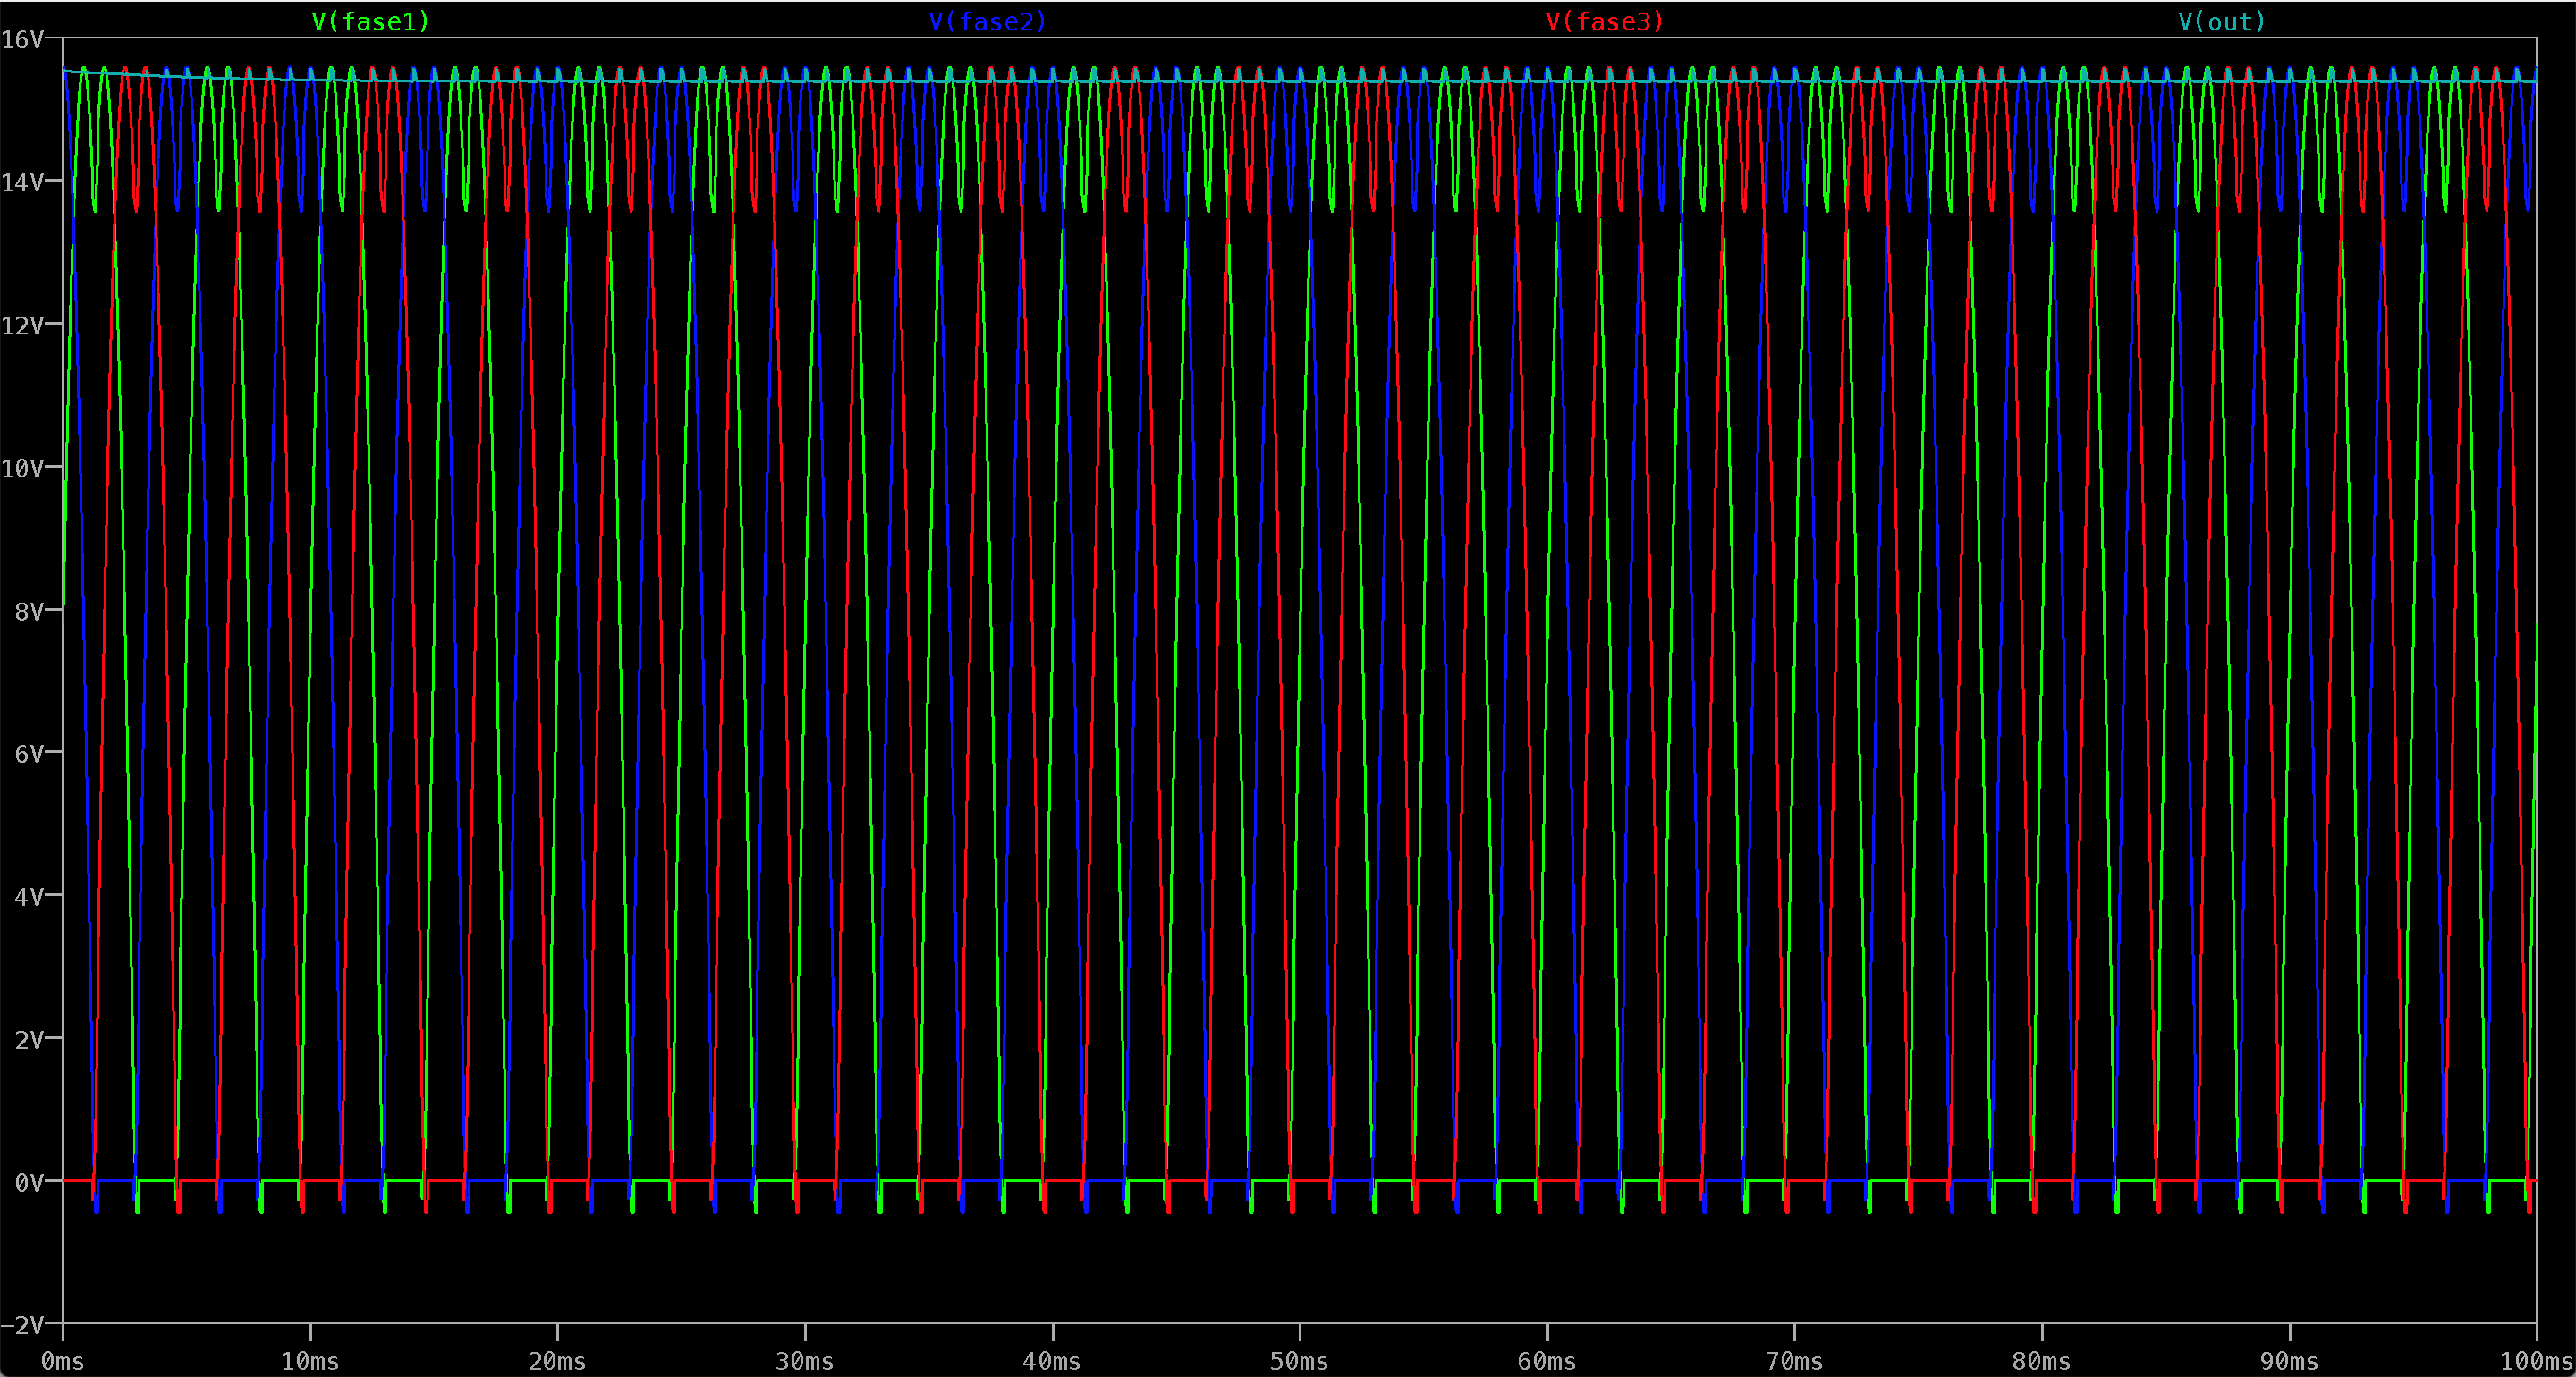
\includegraphics[width=0.9\textwidth]{prens6.png}
  \caption{Resultat af simuleringen. \textcolor{cyan}{$V_{out}$: Målingen over load modstanden}, \textcolor{green}{$V_{fase1}$: Målingen af fase 1}, \textcolor{blue}{$V_{fase2}$: Målingen af fase 2}, \textcolor{red}{$V_{fase1}$: Målingen af fase 1}}
  \label{fig:prens6}
\end{figure}

Det skal nævnes, at skaleringen af komponenter i det simulerede kredsløb ikke er identisk med det tiltænkte. Simuleringen er udført for at konstatere kredsløbets teoretiske funktionalitet.   


Ud fra resultatet\footnote{Se bilag, Timebox 7, for yderligere information.} i simuleringen var vi overbevist om, at kredsløbet i teorien kunne leve op til den ønskede funktionalitet. Næste del af processen var derfor at opbygge kredsløbet på et breadboard i en nedskaleret version.

\subsubsection{Realisering på breadboard (nedskaleret)}
\label{sec:real-pa-breadb}

Kredsløbet blev opbygget på et breadboard i en nedskaleret version for at teste funktionaliteten. Med nedskaleret menes der, at vi benyttede en 1 k$\Omega$’s modstand som load, således der ikke blev trukket en stor strøm gennem kredsløbet. Der blev ligeledes påsat en tilpasset kondensator parallelt med load-modstanden for at udjævne eventuelt \textit{ripple} på outputtet. 

Figur \ref{fig:prens7} viser et skærmbillede fra målingen med oscilloskop af den nedskalerede realisering.

\begin{figure}[h]
  \centering
  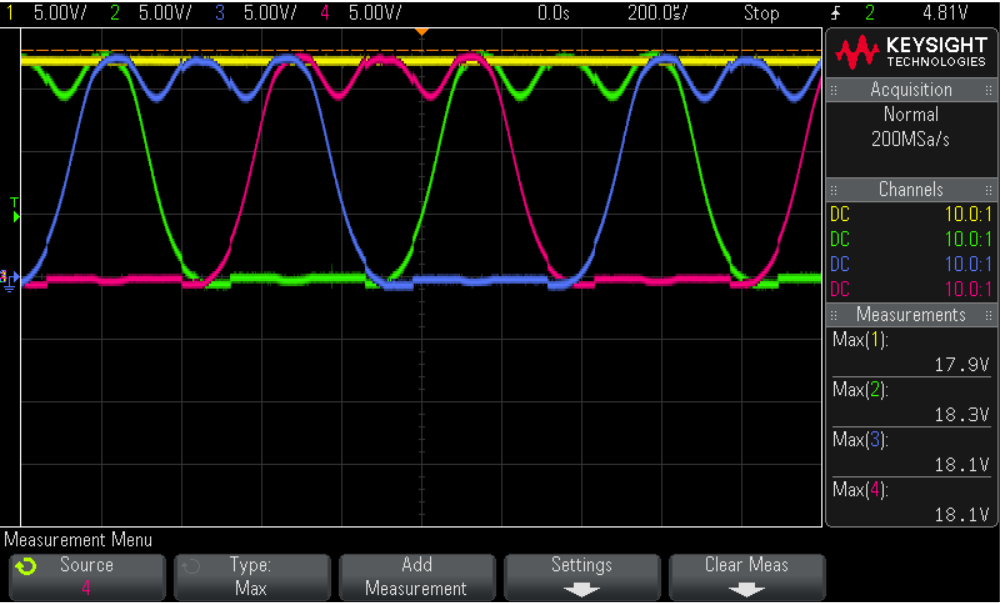
\includegraphics[width=0.8\textwidth]{prens7.png}
  \caption{Nedskaleret realisering på breadboard. Gul: $V_{out}$. Grøn, blå og rød: $V_{in}$ (3 faser)}
  \label{fig:prens7}
\end{figure}

Her ses det, at outputtet er jævnt ensrettet i forhold til de tre faser, hvorved vi kunne konstatere, at det nedskalerede kredsløb fungerede efter hensigten.  

For yderligere at bevise, at den aktive ensretter var væsentlig mere effektiv end en standard diodebro, foretog vi en måling af spændingen på én af MOSFET transistorernes gate pin i forhold til fasen på transistorens \textit{source} pin.

Figur \ref{fig:prens8} viser et skærmbillede af resultatet af målingen. 

\begin{figure}[h]
  \centering
  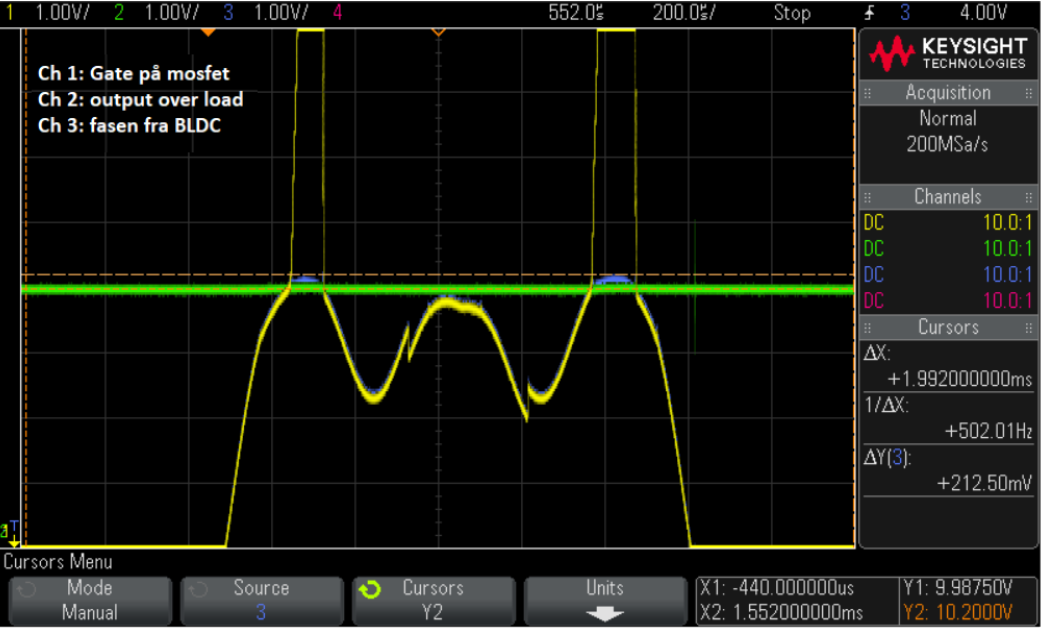
\includegraphics[width=0.8\textwidth]{prens8.png}
  \caption{Måling af gate- vs. source spænding}
  \label{fig:prens8}
\end{figure}

Her ses det, at der er et spændingsfald på 212.5 mV fra gate til source, hvilket er en klar forbedring i forhold til en diodes forward spænding på 700 mV.

Spændingstabet er forårsaget af MOSFET transistorens on resistance, RDS(on), som under denne test var 4$\Omega$. Når kredsløbet skal realiseres uden nedskalering, vil der blive valgt en MOSFET med en langt mindre RDS(on), hvilket teoretisk vil forbedre kredsløbet yderligere.\footnote{Se bilag, Timebox 7, for yderligere information}

\subsection{Spændingsregulator (Jacob)}
\label{sec:spand-jacob}


\subsection{Motorstyring}
\label{sec:motorstyring-1}

\subsubsection{Servo motor og ESC driver (Søren)}
\label{sec:servo-motor-og}

For at få vores servo motoren til at fungere, kræves der et signal på 50 Hz og ved at justere PWM mellem 1 ms til 2 ms aktiv høj, hvilket fremgår fra databladet på servo motoren (SG90 micro servo). Kan vi justere positionen på servo motor fra 0 – 90 grader.

Dette signal bruges også til at justere hastigheden på vores BLDC-motor, via vores ESC. De værdier vi brugte, var 1 ms til stop af BLDC-motor og værdien 1.3 ms, for at kunne starte motoren. Denne værdi 1,3 ms, kom vi frem til via brug af et scope med et wavegen, hvor vi kom frem til at, at ved denne værdi, havde motoren nemt ved at starte. Følgende krav blev opsat, for at vi kunne verificere at det virkede efter hensigten    

\begin{itemize}
\item 50 Hz signal, 20 ms periode (Krav nr. 2.1.3.8.1)
\item Skal kunne justere puls mellem 1 – 2 ms. (Krav nr. 2.1.3.8.2)
\end{itemize}
\clearpage
\begin{figure}[h]
  \centering
  \lstinputlisting[language=c,firstline=39,lastline=101,basicstyle=\scriptsize\ttfamily]{./kode/servo-driver.cpp}  
  \caption{Opsætning af servo og ESC driver}
  \label{fig:kodes1}
\end{figure}

\clearpage
Ved at opsætte analog Discovery til på pin PTD3, vises at vores init funktion virker efter hensigten, med 50 Hz og 1 ms puls. Og hermed lever op til følgende krav 2.1.3.8.1 og 2.1.3.8.2, der er beskrevet på forrige side.

\begin{figure}[h]
  \centering
  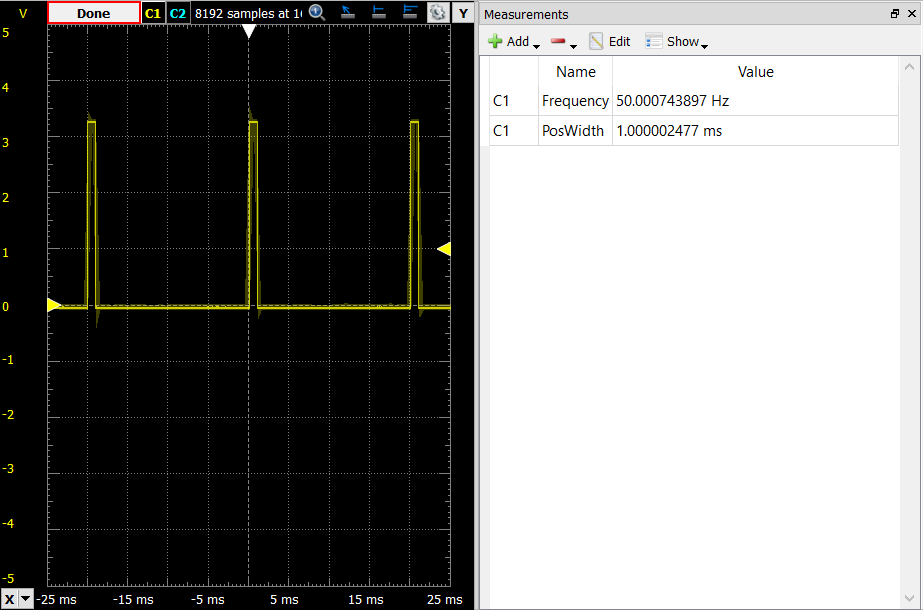
\includegraphics[width=0.8\textwidth]{mots4.png}
  \caption{Test af init-funktion}
  \label{fig:mots4}
\end{figure}

Herefter har vi implementeret en funktion til at styre vores servo motor. Den tager et argument, som er i procent, hvor meget den skal dreje, i forhold til om den skal give fuld gas (100\%) eller bare kører i tomgang (0\%). Men da vi fik monteret servo motor, fik vi testet at ved 1,4 ms signal til servo, at dette var fuldgas, dette blev derefter tilpasset i koden. Så vores max værdien der kunne sendes ud er 1,4 ms.

\begin{figure}[!htb]
    \centering
    \begin{minipage}{.5\textwidth}
        \centering
  \lstinputlisting[language=c,firstline=102,lastline=107,basicstyle=\scriptsize\ttfamily]{./kode/servo-driver.cpp}
  \label{fig:kodes2}
    \end{minipage}%
    \begin{minipage}{0.5\textwidth}
        \centering
        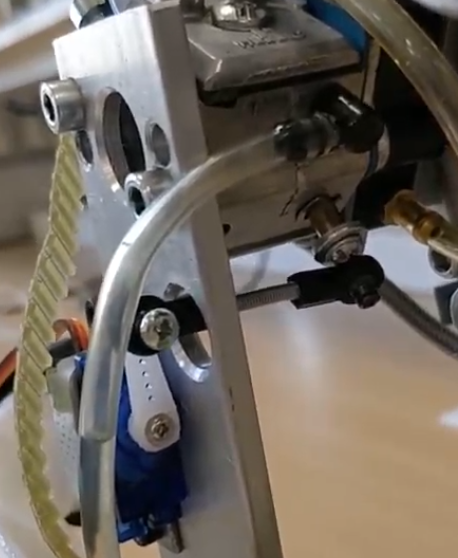
\includegraphics[width=0.8\linewidth]{mots5.png}
        \label{fig:mots5}
    \end{minipage}
    \caption{Kode til at styre gasspjældet}
  \end{figure}

\subsubsection{Start af motoren}
\label{sec:start-af-motoren}

Da den driver vi brugte til at styre servo motoren er den samme, som vi skal bruge for at kunne få vores BLDC-motor i gang, da den fungere som el-starter til motoren. Blev der implementeret en pin ekstra, i driveren, der er vist i koden se figur \ref{fig:kodes3}. Herefter lavede vi en start funktion, der skulle bruges til at starte motoren.

Flow for opstart af motor, ved funktionen \lstinline{start()}:

\begin{enumerate}
\item Startknap initialiseres
\item Afventer at brugeren trykker på knappen
\item En timer opsættes, som tæller vores ’i’ værdi op, når der er gået 500 ms.
\item Så prøver motoren at starte benzinmotoren, og det vil den gøre så længe start knappen er trykket ned (dog i maks. 15 sek)
\item Efter 15 sek vil opstartsprocessen afbrydes.
\end{enumerate}

\begin{figure}[h]
  \centering
  \lstinputlisting[language=c,firstline=132,lastline=153,basicstyle=\scriptsize\ttfamily]{./kode/servo-driver.cpp}  
  \caption{Kode til \lstinline{start()}}
  \label{fig:kodes3}
\end{figure}

\begin{figure}[h]
  \centering
  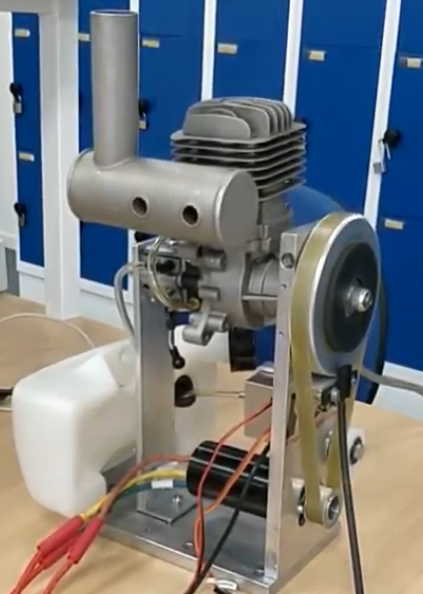
\includegraphics[width=0.8\textwidth]{mots6.png}
  \caption{BLDC-motor forbundet til motoren med en tandrem}
  \label{fig:mots6}
\end{figure}

\subsubsection{RPM-detektering}
\label{sec:rpm-detektering}

Implementering af koden til at aflæse rpm, der skal bruges til vores PID-regulering. Har vi taget udgangspunkt i at aflæse et tacho signal som kommer fra vores tændspole. Dette signal lave en høj spænding ved hver omdr, og går lav igen. 

For at afkode dette signal, bruges der input capture, der er implementeret i TPM periferenheden på kl25. Funktionen input capture, fungere ved at den tælle op til hver ’rising edge’ og gemmer denne værdi. Og når vi kender værdien og frekvensen vi tæller op med, kan vi omregne dette til RPM. 

Ved formlen: $60 \mathrm{sek} \cdot \frac{\mathrm{frekvens}}{\mathrm{input\ capture\ værdien}}=\mathrm{RPM}$.

Selve koden er vist her forneden, hvor vi bruger interrupts, til at opfange overflows og når vi får et rising edge, gemmer den værdi i CNV-registeret.

\begin{figure}[h]
  \centering
  \lstinputlisting[language=c,firstline=39,lastline=58,basicstyle=\scriptsize\ttfamily]{./kode/rpm-detect.cpp}  
  \caption{Kode til RPM-detektering}
  \label{fig:kodes3}
\end{figure}

Her initialiseres vores TPM1 modul. Vores frekvens der bruges til at tælle op med, bliver nedskaleret, til 375 kHz. Dvs. imellem hver overflows går der 5,75 Hz, hvilket passer med vores måle område (17 - 167 Hz) vi arbejder i.

\subsubsection{Stepinput og overføringsfunktion (Simon)}
\label{sec:tests}

PID-koefficienterne skal defineres udfra en overføringsfunktion for vores system som skal reguleres. For at udlede overføringsfunktionen blev et forsøg med optagelse af steprespons udarbejdet.

% Et testprogram kan køres via microcontroller som foretager PID-reguleringen og optage motorens omdrejninger ved forskellige skift mellem hastigheder. Disse gentages for forskellige værdier af $K_p$ og $K_i$.

Som udgangspunkt skulle det interessante for dronecopteren være at % I en teststand vil formålet være at test forskellige værdier af koefficienterne og i forskellige kombinationer. Målet med PID-reguleringen er at
strømmen fra batteri til dronens propelmotorer er konstant. Tilgengæld skal spjældet til forbrændingsmotoren konstant reguleres. Derfor vil en teststand som udgangspunkt have følgende:
\begin{itemize}
\item input: strøm fra batteri til drone
\item output: regulering af spjæld via servomotor
\end{itemize}

Her vil $e(t)$ være et mål for forskellen mellem den ønskede strømstyrke og den faktiske.

Det var ikke muligt at måle strømmen fra batteri til drone. For at lave en teststand som kan tjene som demonstration af PID-regulering samt som skabelon for senere tests fremstilles istedet en teststand som skal justere spjældet i forhold til motorens omdrejninger. Dvs:

\begin{itemize}
\item input: motorens omdrejninger
\item output: regulering af spjæld via servomotor
\end{itemize}

I dette tilfælde vil $e(t)$ være et mål for forskellen mellem det ønskede omdrejningstal og det faktiske.

For at få en grov ide om niveauet af koefficienterne kan en simulink simulation være gunstig. I denne skal gøres en række antagelser af forholdet mellem spjældvinkel og omdrejningstallet. Når koefficienterne er tunet i simulink kan der laves en test.

% I testen skal der laves forskellige trinsvise ændringer af omdrejningstallet. Fjare\autocite{pid1} har beskrevet hvordan 4 forskellige trinmønstre (se figur\ref{fig:paths}) blev brugt til at justere en PID-algoritme som blev brugt til en forbrændingsenhed i en ubemandet flyvende enhed.

% \begin{figure}[h]
%   \centering
%   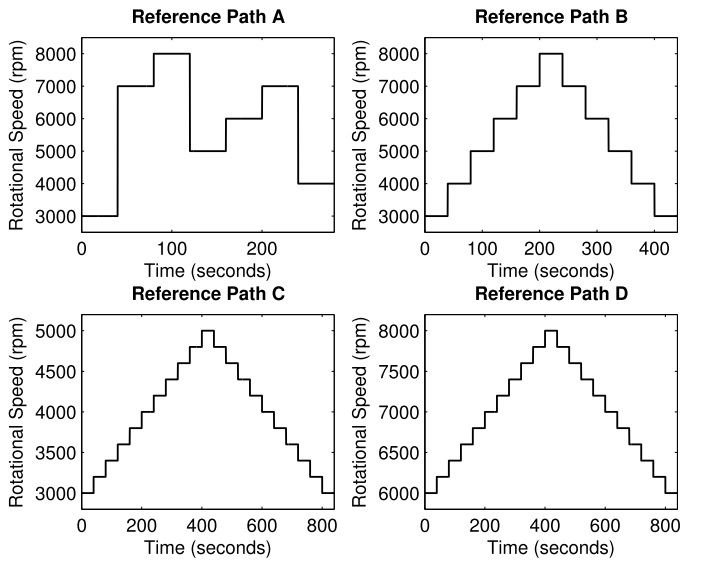
\includegraphics[width=0.7\textwidth]{refpaths.JPG}
%   \caption{Trinmønstre}
%   \label{fig:paths}
% \end{figure}

% På trods af at forbrændingsenheden altså ikke opladet batteri virker det relevant at tage udgangspunkt i lignende trinmønste til PID-kontrol af motoromdrejninger.

% KL25 vil tjene både som microcontroller og datalogger.

\myparagraph{Steprespons}
\label{sec:steprespons}

%For at simplificere PID-reguleringen forsøges forst med regulering af spjæld i forhold til motorens omdrejninger.
Der vil tages udgangspunkt i måling af et steprespons på motorens omdrejninger. Til målinger af omdrejninger anvendtes et oscilloskop som optog data fra Hall-sensoren. Optagelsen blev tricket fra KL25Z.% foreslås at bruge Pocketbeagle som vil kunne foretage måling af omdrejninger via Hall-sensor og lagre data i en fil som kan eksporteres til analyse i Matlab.

Data fra oscilloskopet bestod i 50000 målinger som bestod af Hall-sensorens spænding, spændingen fra servomotoren, der styrer spjældet, samt et tidsmål. Nedenfor ses et udsnit af de 50000 målinger:

\begin{table}[h]
  \centering
% BEGIN RECEIVE ORGTBL tabel4
\begin{tabular}{r|r|r}
\hline
\textbf{second} & \textbf{Volt} & \textbf{Volt1} \\
\hline
-1 & 0.215206000000000 & 4.98492460000000 \\
-0.999900000000000 & 0.215206000000000 & 4.90452260000000 \\
-0.999800000000000 & 0.134804000000000 & 4.90452260000000 \\
-0.999700000000000 & 0.215206000000000 & 4.98492460000000 \\
-0.999600000000000 & 0.215206000000000 & 4.90452260000000 \\
-0.999500000000000 & 0.215206000000000 & 4.90452260000000 \\
-0.999400000000000 & 0.215206000000000 & 4.90452260000000 \\
-0.999300000000000 & 0.215206000000000 & 4.82412060000000 \\
-0.999200000000000 & 0.215206000000000 & 4.90452260000000 \\
\hline
\end{tabular}
% END RECEIVE ORGTBL tabel4
  \caption{}
  \label{tab:komp3}
\end{table}
\begin{comment}
#+ORGTBL: SEND tabel4 orgtbl-to-latex :splice nil :skip 0
|--------------------+-------------------+------------------|
|             second |              Volt |            Volt1 |
|--------------------+-------------------+------------------|
|                 -1 | 0.215206000000000 | 4.98492460000000 |
| -0.999900000000000 | 0.215206000000000 | 4.90452260000000 |
| -0.999800000000000 | 0.134804000000000 | 4.90452260000000 |
| -0.999700000000000 | 0.215206000000000 | 4.98492460000000 |
| -0.999600000000000 | 0.215206000000000 | 4.90452260000000 |
| -0.999500000000000 | 0.215206000000000 | 4.90452260000000 |
| -0.999400000000000 | 0.215206000000000 | 4.90452260000000 |
| -0.999300000000000 | 0.215206000000000 | 4.82412060000000 |
| -0.999200000000000 | 0.215206000000000 | 4.90452260000000 |
|--------------------+-------------------+------------------|
\end{comment}

Spændingen fra Hall-sensoren, Volt1, anvendes.
Når data plottes for et kort tidsrum ses støj omkring 5 volt

\begin{figure}[h]
  \centering
  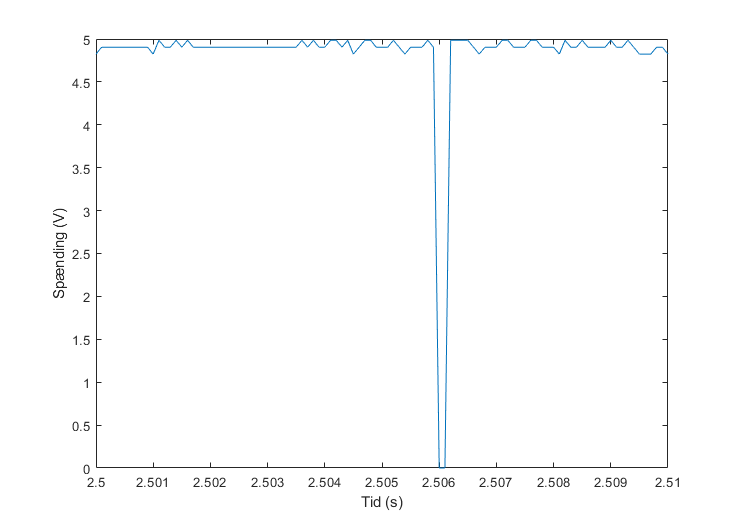
\includegraphics[width=0.6\textwidth]{mo1.png}
  \caption{}
  \label{fig:mo1}
\end{figure}

Data processeres nu med følgende Matlab-script:
\begin{lstlisting}[language=Matlab]
close all
data = stepdata5;
t = data.second;
v = data.Volt1;
border1 = 4.5;
border2 = 0.1;
v2 = data.Volt;
b = 0;
stop = 0;
tp = [];
tpt = [];
vpt0 = [];
i = 1;
nyv = [];
while (i <= length(t))
    if (v(i)>border1)
        vn = 5;
    else
        vn = 0;
    end
    nyv = [nyv vn];
    i = i + 1;
end
i = 1;


while (i < length(t))
    if ((nyv(i+1)>border1 & nyv(i)<border2) & b == 0)
        t1 = t(i+1);
        stop = 1;
        b = 1;
    end
    i = i + 1;
    vpt0 = [vpt0 0];
    while (stop ~= 2 & b == 1 & i < length(t))
        if (stop == 1)
            while (stop ~= 2 & i < length(t))
                if (nyv(i+1)>border1 & nyv(i)<border2)
                    t2 = t(i+1);
                    stop = 2;
                end
                i = i + 1;
                vpt0 = [vpt0 0];
            end
        end
        if (stop == 2)
            period = t2-t1;
            tpt = [tpt t2];
            vpt0(i) = nyv(i);
            tp = [tp period];
            t1 = t2;
            stop = 1;
        end
    end
end  
\end{lstlisting}

I scriptet fortolkes spænding over 4,5 V som 5 V. Markering af periodegrænser ved 5 Volt kan ses her (de røde prikker øverst):

\begin{figure}[h]
  \centering
  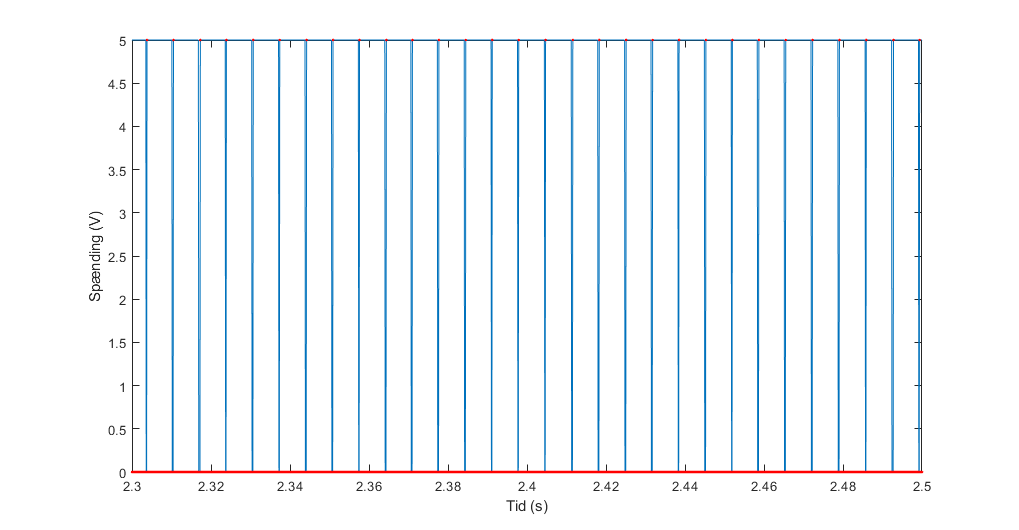
\includegraphics[width=0.6\textwidth]{mo2.png}
  \caption{}
  \label{fig:mo2}
\end{figure}

Herudover udregnes tiden for hver omdrejningsperiode og gemmes i vektoren ”tp”.
Ved plot at tp givet ved rpm overfor tid fås:

\begin{figure}[h]
  \centering
  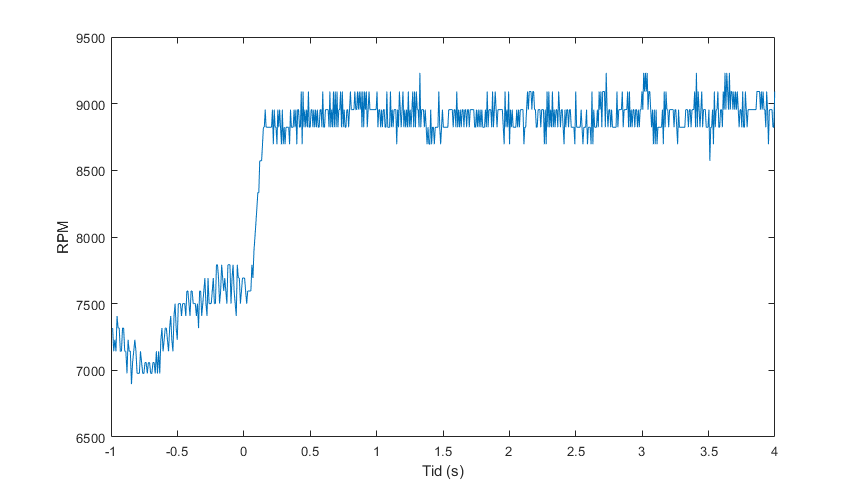
\includegraphics[width=0.6\textwidth]{mo3.png}
  \caption{}
  \label{fig:mo3}
\end{figure}

\myparagraph{Overføringsfunktion}

\label{sec:overforingsfunktion}
Udfra stepresponset skal følgende identificeres:

\begin{itemize}
\item Rise time, $t_r$
\item Settling time, $t_s$
\item Overshoot, $M_p$
\item Peak time, $t_p$
\end{itemize}

Scopet der har målt data gemmer også data op til stepresponset. Stepresponset ses ved tiden 0.
Ved at applicere et midlingsfilter på 200 fås et indtryk af et steady-state niveau ved 8900, med start fra 7600, dvs 1300. 

\begin{figure}[h]
  \centering
  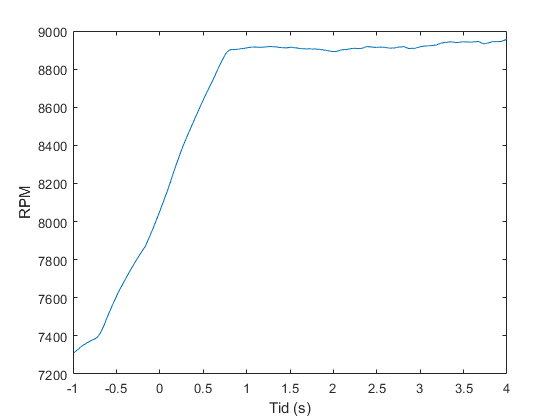
\includegraphics[width=0.5\textwidth]{mo4.png}
  \caption{}
  \label{fig:mo4}
\end{figure}

Ved at applicere et midlingsfilter på 10 fås et indtryk af en 1. grads overføringsfunktion.

\begin{figure}[h]
  \centering
  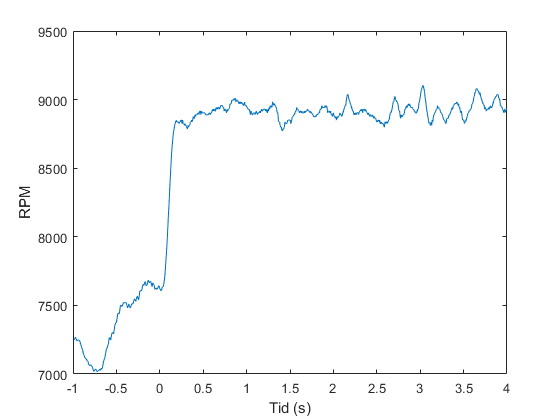
\includegraphics[width=0.5\textwidth]{mo5.png}
  \caption{}
  \label{fig:mo5}
\end{figure}

Det måles at steady-state er opnået ved 0,19 sekunder. Dvs. $0.81 = 5\tau \Leftrightarrow \frac{0,19}{5}=\tau=0,04$.

Hermed kan overføringsfunktionen sættes som
\begin{equation}
  \label{eq:1}
G(s) = \frac{1300}{0,04s+1}  
\end{equation}

% I sidste timebox fandtes overføringsfunktionen
% \begin{equation}
%   \label{eq:1}
% G(s) = \frac{8900}{0,04s+1}  
% \end{equation}
\clearpage
I Simulink oprettes følgende:

\begin{figure}[h]
  \centering
  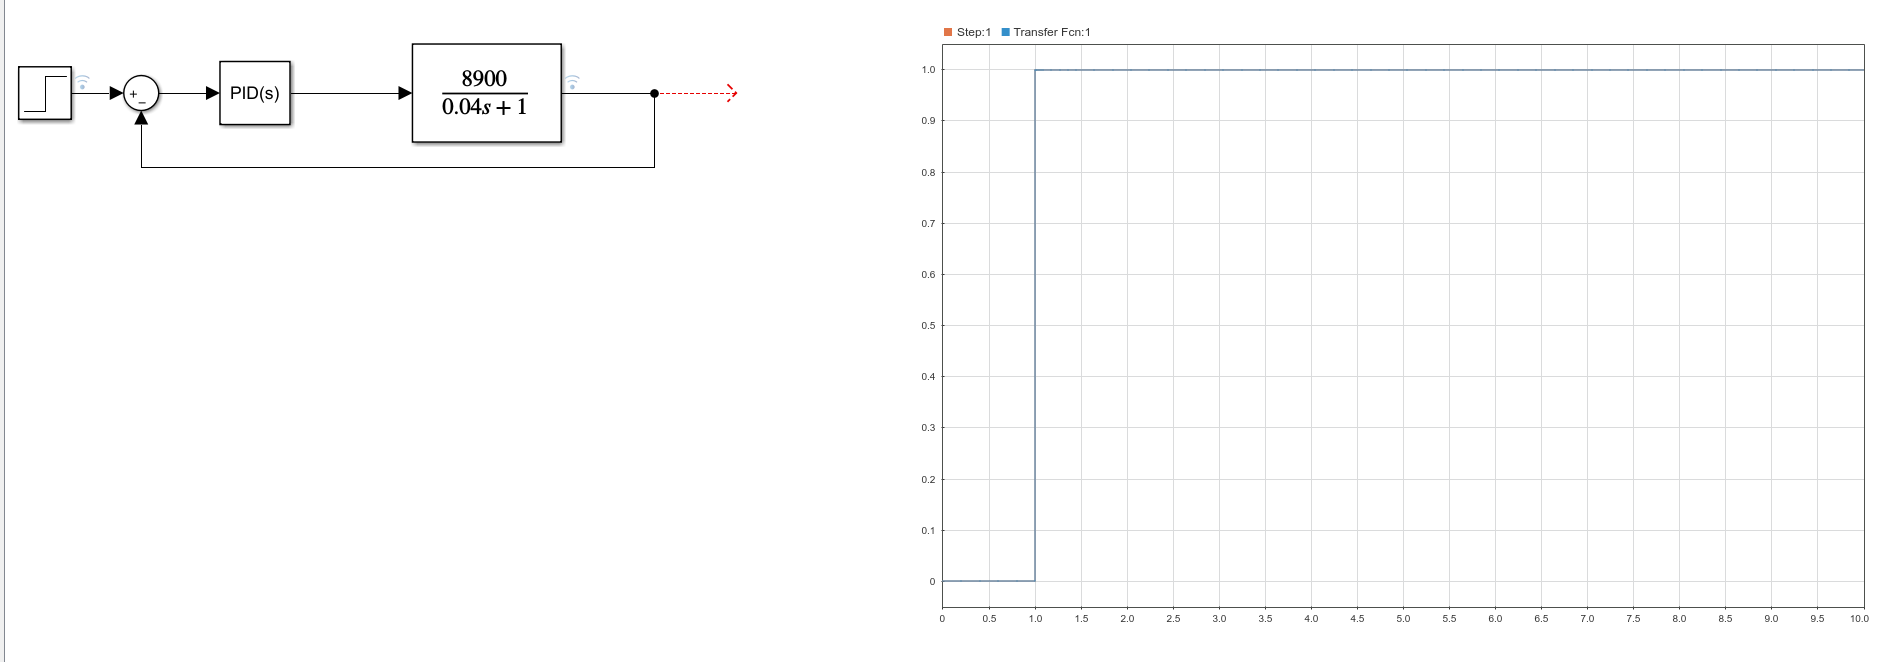
\includegraphics[width=0.6\textwidth]{sbil1.png}
  \caption{Simulink - diagram}
  \label{fig:sbil1}
\end{figure}

Herefter laves autotuning i PID-modulet. Der findes koefficienter svarende til $P=0,0010$, $I=0,0514$, $D=-1,4946$ og følgende respons:

\begin{figure}[h]
  \centering
  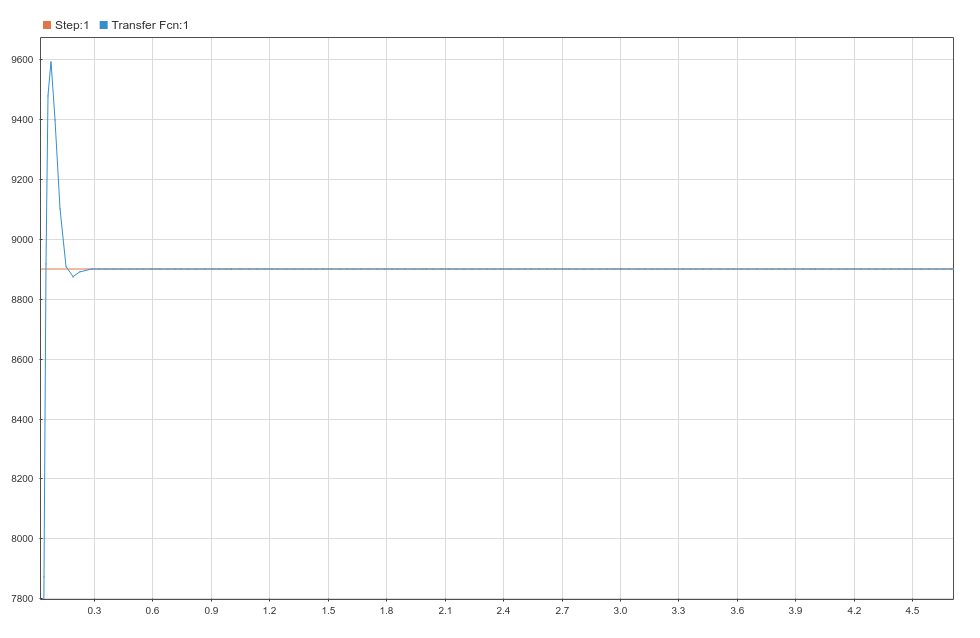
\includegraphics[width=0.6\textwidth]{sbil2.png}
  \caption{Simulink - diagram 2}
  \label{fig:sbil1}
\end{figure}

\subsubsection{Software (Simon)}
\label{sec:software-1}

Der udarbejdes nu et udkast til PID-kontrol software som også benytter sig af software til kontrol af servomotor samt aflæsning af motorens omdrejninger (se afsnit XXX).

\begin{lstlisting}[language=C,basicstyle=\ttfamily]
#include <stdio.h>
#include "board.h"
#include "peripherals.h"
#include "pin_mux.h"
#include "clock_config.h"
#include "MKL25Z4.h"
#include "fsl_debug_console.h"
#include "rpm-detect.h"
#include "servo_driver.h"

// Filtrering
double alpha = 0.2;
double measuredSpeed = 0 ;

// Koefficienter
double kp = 0.001;
double ki = 0.0514;
double kd = -1.4946;
double K1;
double K2;
double K3;

// Vægtning af koefficienter
double setpointWeight = 0.2;
double lowpassSpeed;
double setpointSpeed;

// Diverse
double output;
double throttleopen = 1.0;
float throttlePos;

int rpmch;
int MAX_RPM = 9000;

// Initialiering
double lastSetpointSpeed = 0;
double lastMeasuredSpeed = 0;
double lastLowpassSpeed = 0;
double lastOutput = 0;
double lastLastMeasuredSpeed = 0;

void velPID (int setpointSpeed, int measuredSpeed) {
    lowpassSpeed = alpha * lastLowpassSpeed + (1-alpha ) * measuredSpeed;
    K1 = kp * setpointWeight * (setpointSpeed-lastSetpointSpeed) + kp * (lastMeasuredSpeed-lowpassSpeed);
    K2 = ki * (setpointSpeed-lowpassSpeed);
    K3 = kd * (2 * lastMeasuredSpeed-lowpassSpeed-lastLastMeasuredSpeed);
    output = lastOutput-K1-K2-K3;
    if (output < 0) {
      output = 0;
    }
    throttlePos = output/MAX_RPM;
    lastLowpassSpeed = lowpassSpeed;
    lastLastMeasuredSpeed = lastMeasuredSpeed;
    lastMeasuredSpeed = lowpassSpeed;
    lastSetpointSpeed = setpointSpeed;
    lastOutput = output;
    angle_throttle(throttlePos);
}

init_read_rpm()

int main(void) {
  /* Init board hardware. */
  BOARD_InitBootPins();
  BOARD_InitBootClocks();
  BOARD_InitBootPeripherals();
  /* Init FSL debug console. */
  BOARD_InitDebugConsole();
  rpmch = 7000;
  init_pwm();
  start();
  velPID(rpmch, measuredSpeed);
  return 0 ;
}

\end{lstlisting}


% Udfra disse mål kan der gives et bud på en overføringsfunktion. I matlab kan der via simulink og en overføringsfunktion findes PID-koefficienter og laves tuning. I slutningen af arbejdet undersøges om følgende kravene overholdes:
% \begin{itemize}
% \item Overshoot skal ikke være mere en 197 rpm.
% \item Justeringstiden må max være 8,8 sekunder.
% \item Ifm. et step respons skal 90 \% af målet være opnået i mindre end 3 sekunder.
% \end{itemize}

% Der er tidligere blevet lavet målinger ved steprespons af forbrændingsmotor. 

\clearpage
\section{Resultater}
\label{sec:resultater}

\subsection{Aktiv ensretter}
\label{sec:aktiv-ensretter}

 OBS** Den røde tråd
 \begin{itemize}
 \item Max strøm dronebehov
 \end{itemize}


\subsection{Motorstyring}
\label{sec:motorstyring-2} 

Der blev lavet implementering af PID-koden. Resultatet var desværre at der ved øgning af mindskning af omdrejningstal blev lavet en stigning i omdrejningstal og omvendt.


% \bibliographystyle{unsrt}

\clearpage
\appendix
\addcontentsline{toc}{section}{Bilag}
\vspace*{\fill}
\begin{center}
\Huge{  \textbf{BILAG}}
\end{center}
\vspace*{\fill}

% \appendixpage
% \addappheadtotoc

\addcontentsline{toc}{section}{Timebox 1}
\label{sec:timebox-1}
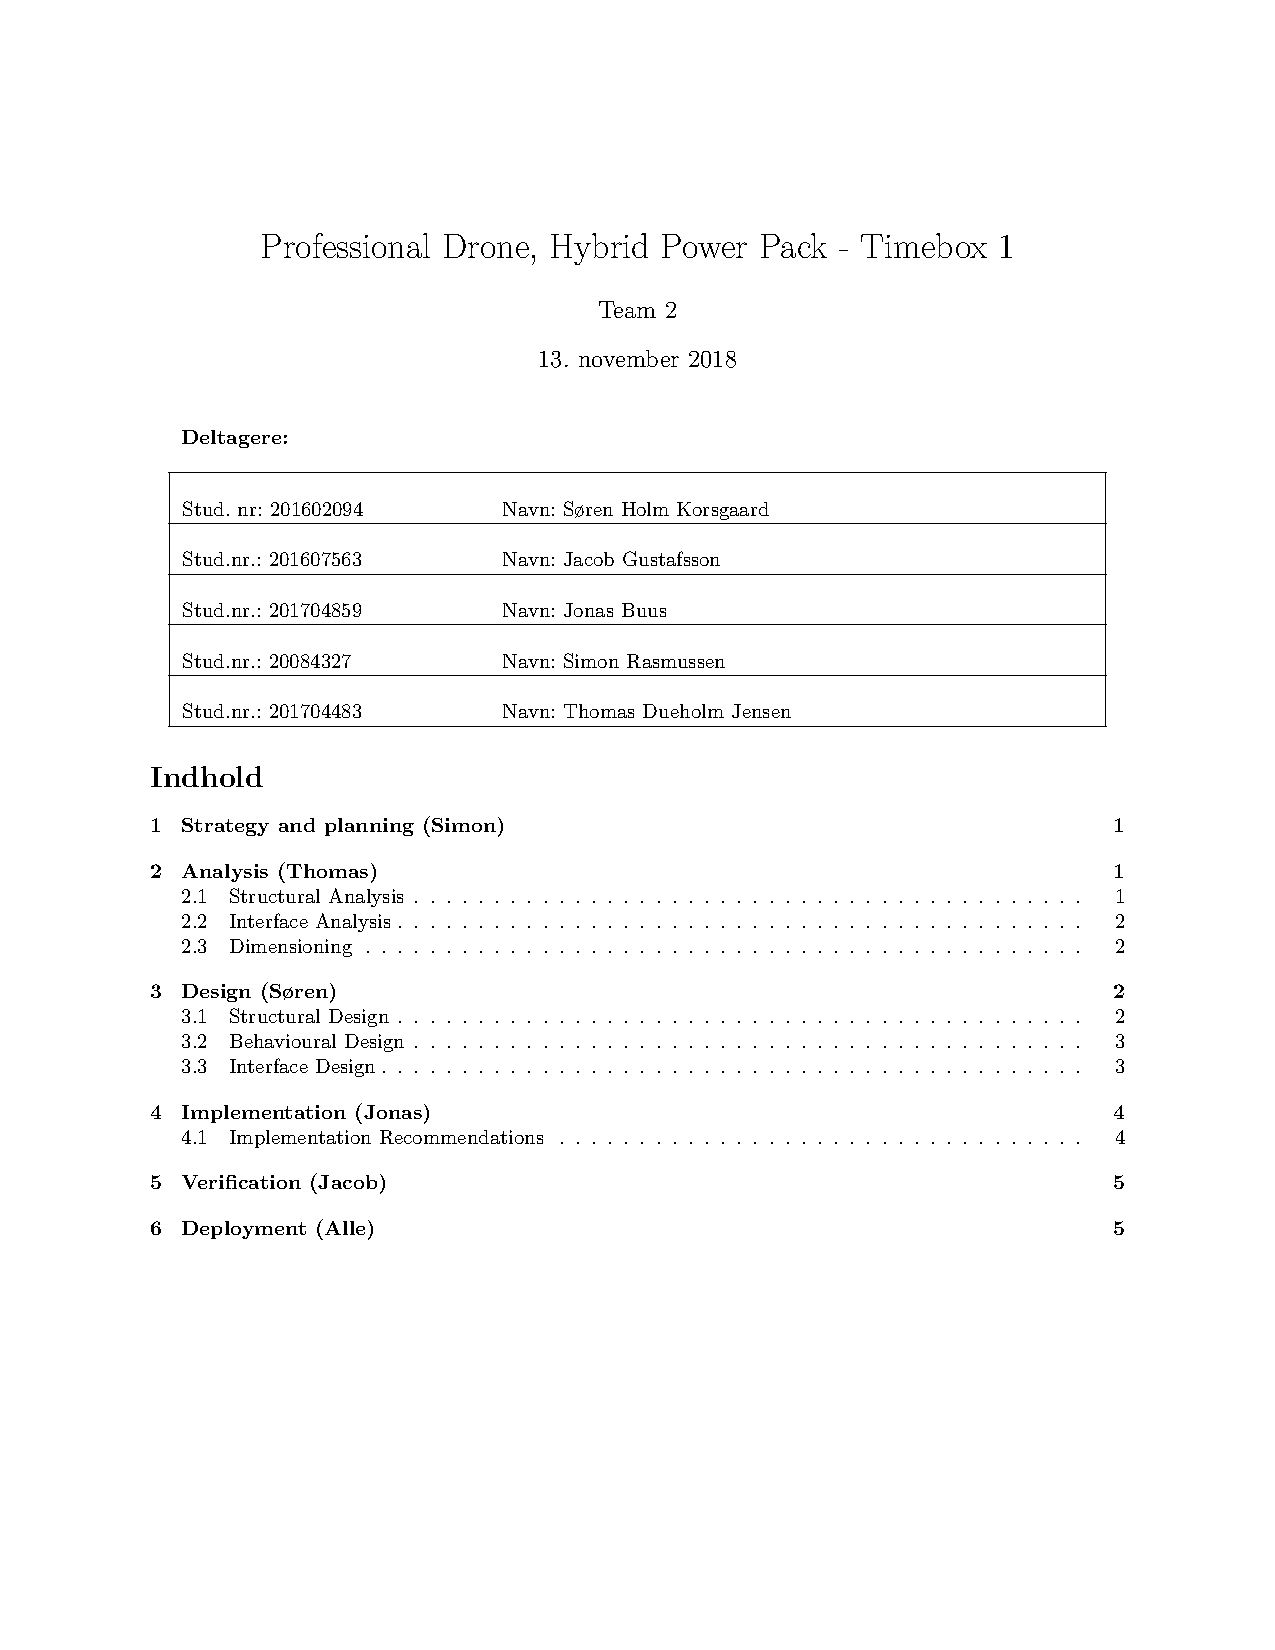
\includepdf[pages={-1}]{timebox1-131118}
\clearpage

\addcontentsline{toc}{section}{Timebox 2}
\label{sec:timebox-2}
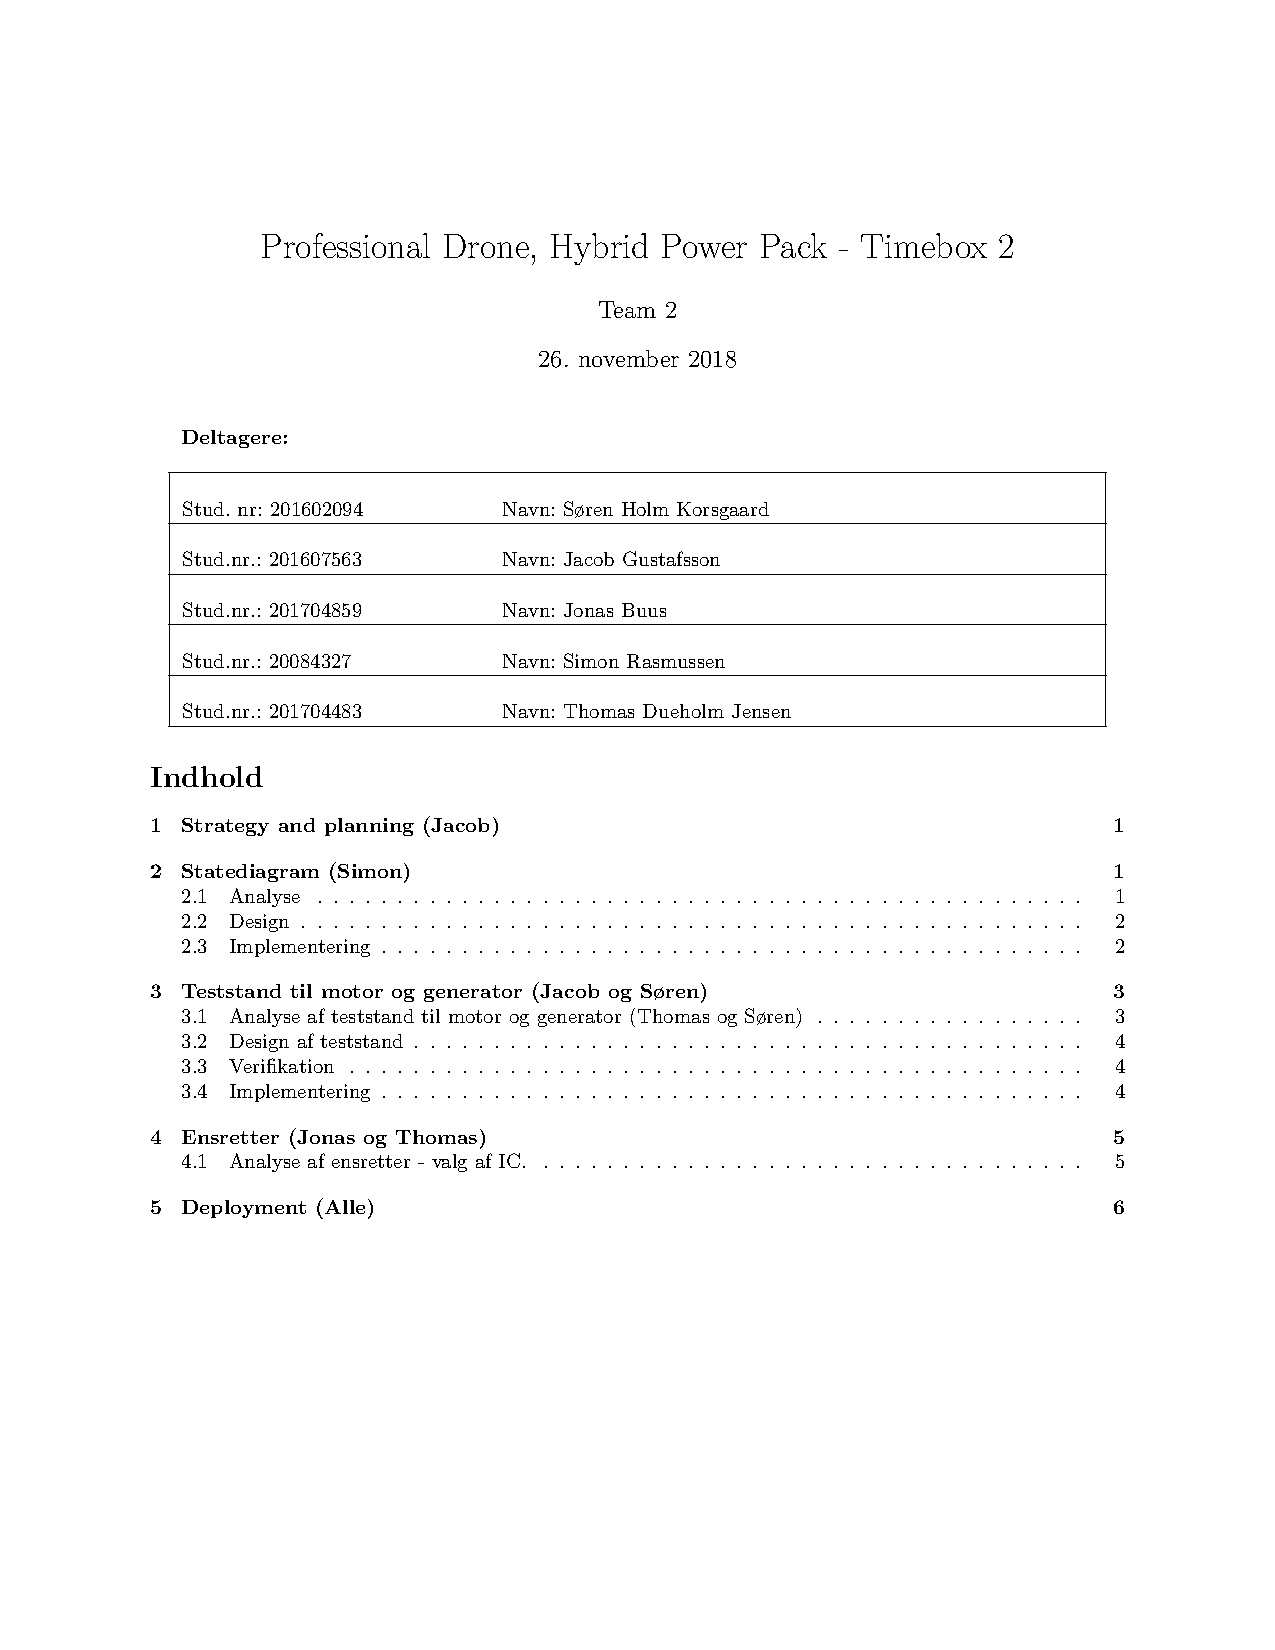
\includepdf[pages={-1}]{timebox2-rettelse-fra-klaus(031218)}
\clearpage

\addcontentsline{toc}{section}{Timebox 3}
\label{sec:timebox-3}
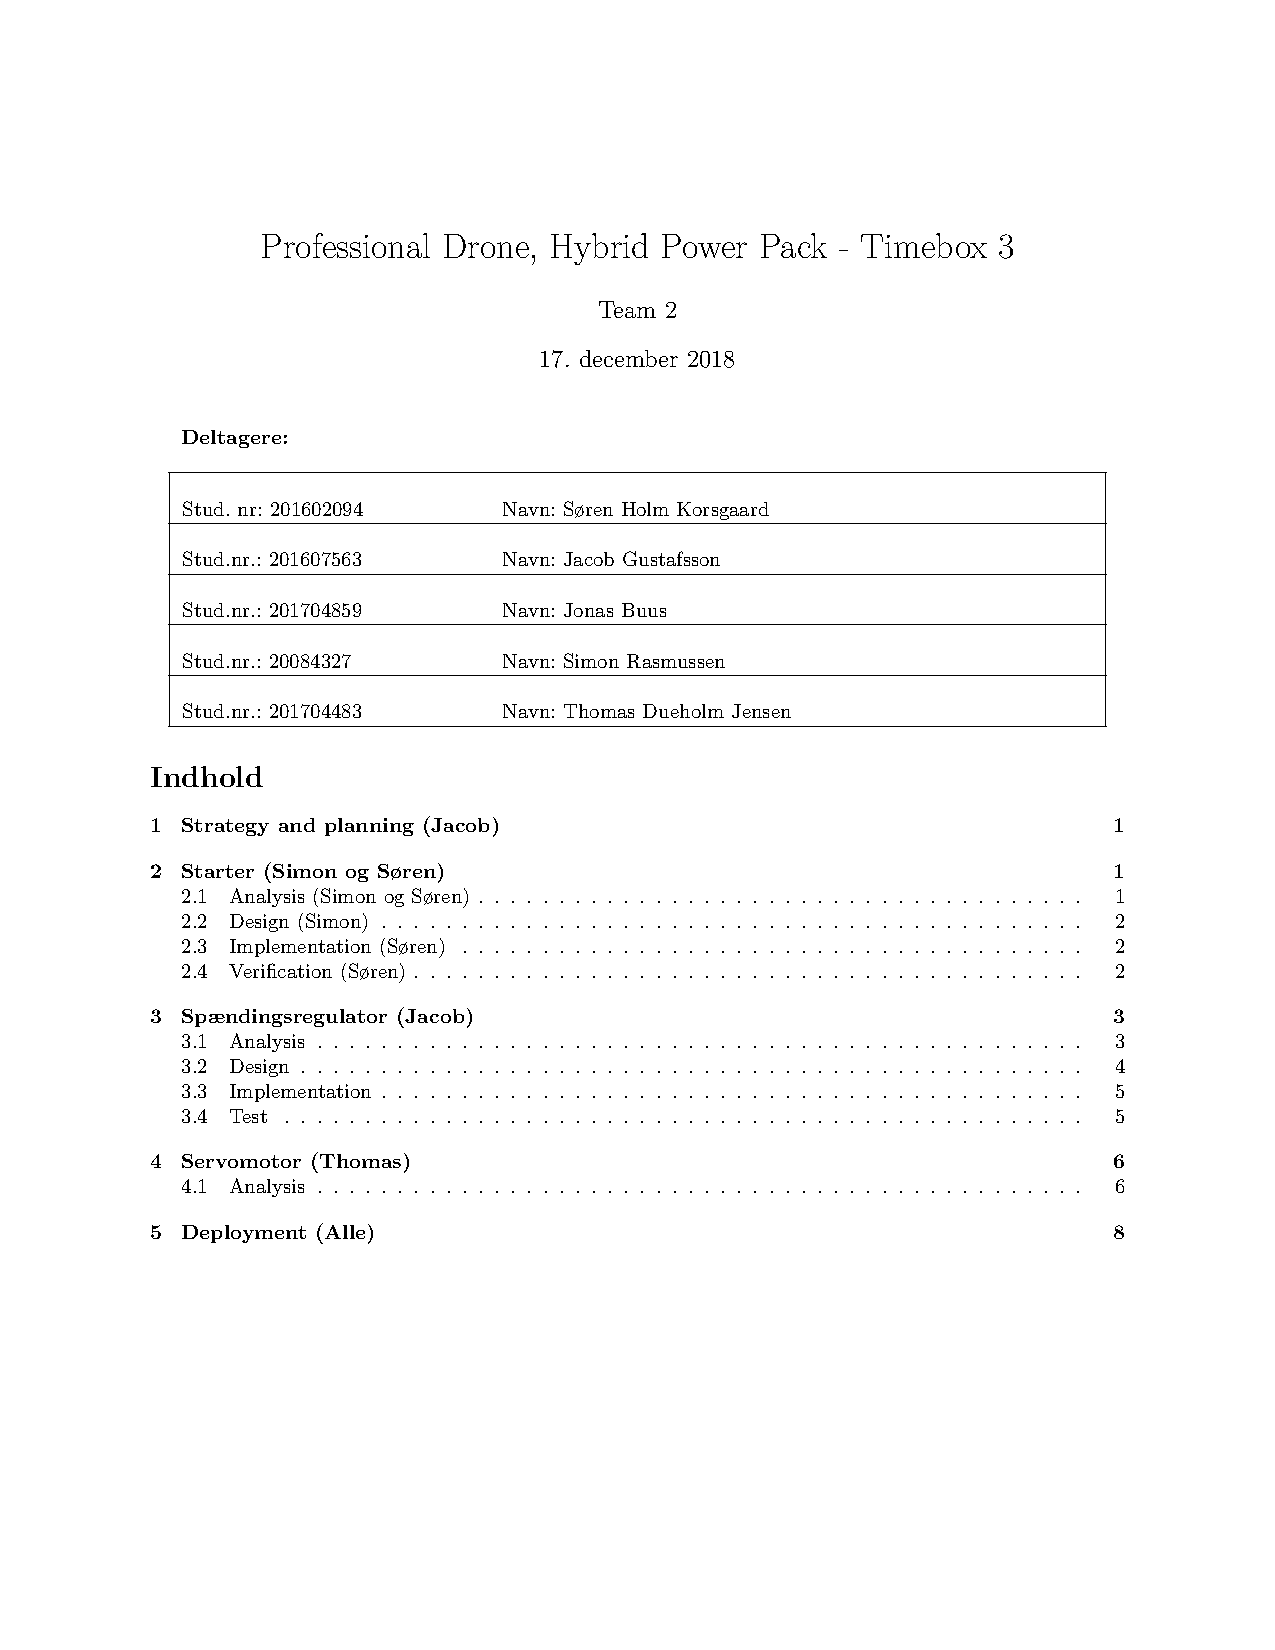
\includepdf[pages={-1}]{timebox3-171218}
\clearpage

\addcontentsline{toc}{section}{Timebox 4}
\label{sec:timebox-4-1}
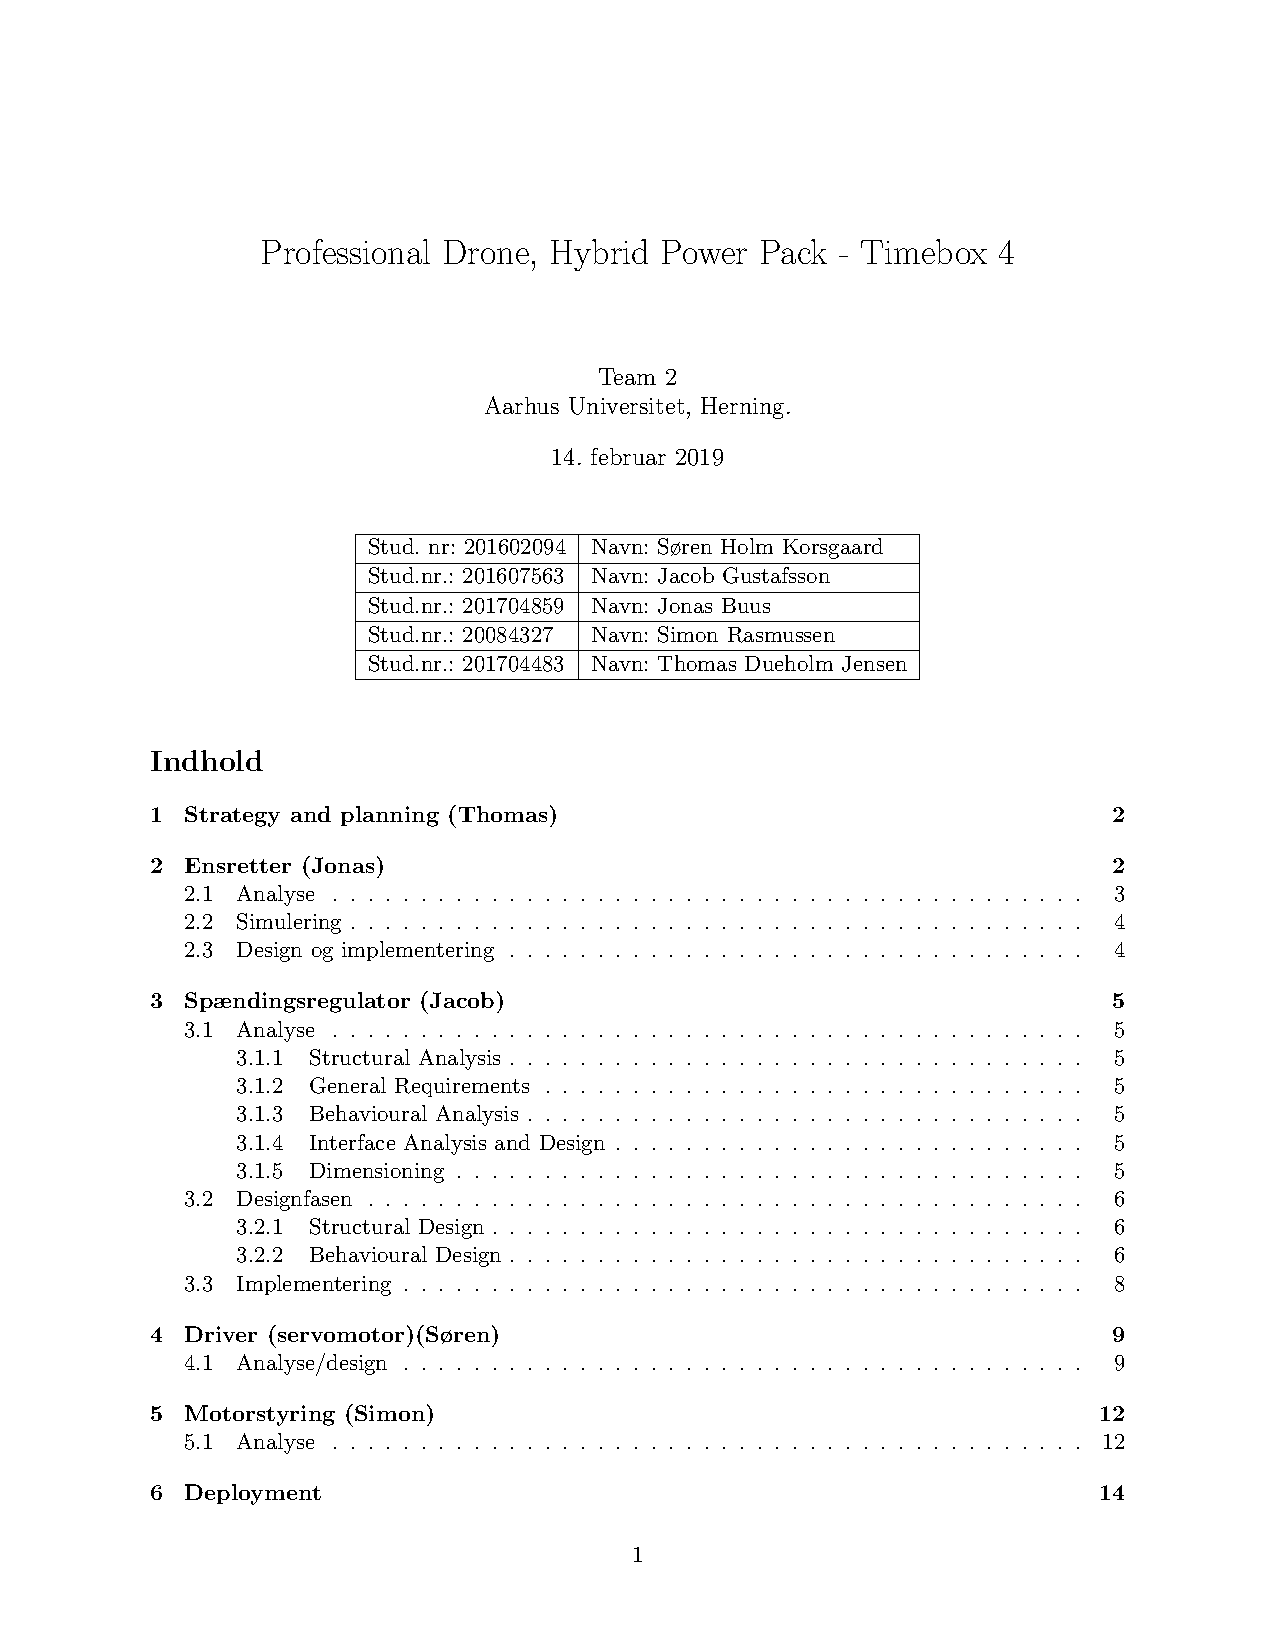
\includepdf[pages={-1}]{timebox4-140219}
\clearpage

\addcontentsline{toc}{section}{Timebox 5}
\label{sec:timebox-5}
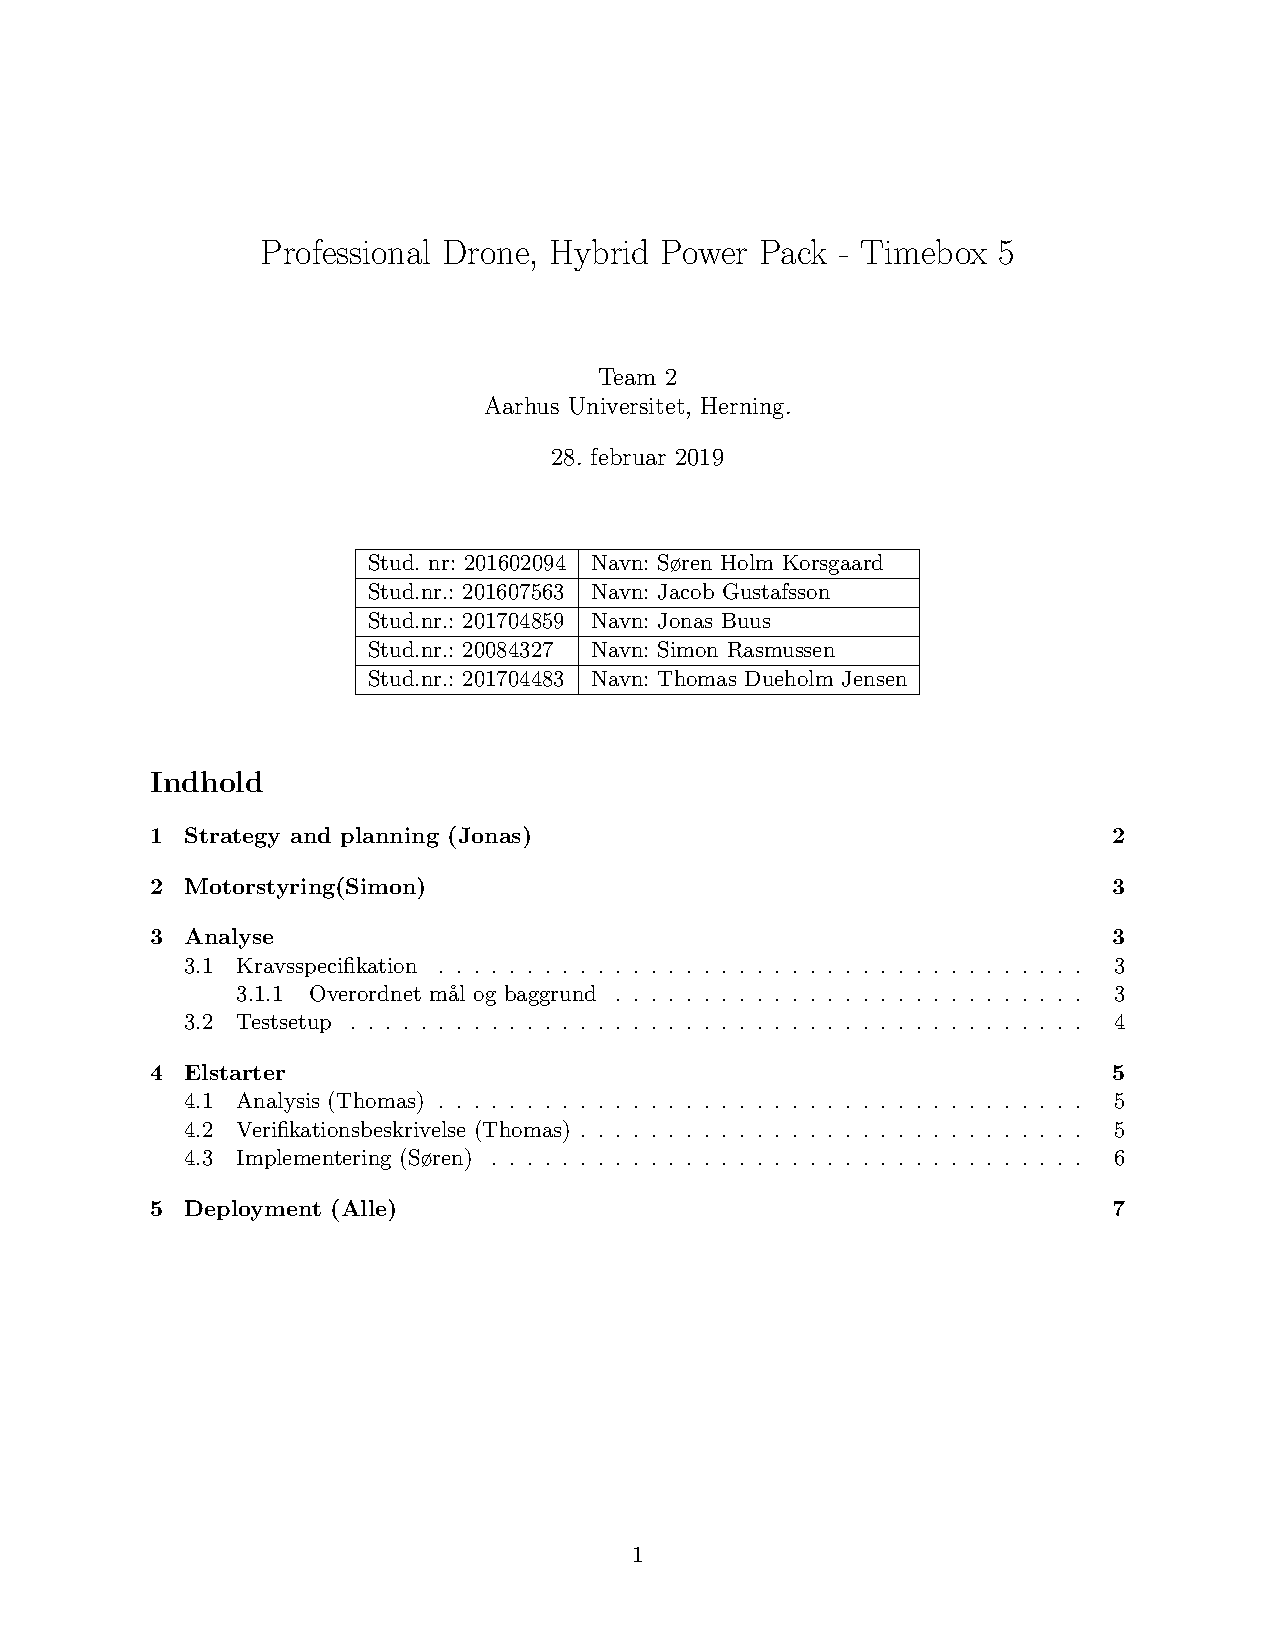
\includepdf[pages={-1}]{timebox5-280219}
\clearpage

\addcontentsline{toc}{section}{Timebox 6}
\label{sec:timebox-6}
\includepdf[pages={-1}]{timebox6}
\clearpage

\addcontentsline{toc}{section}{Timebox 7}
\label{sec:timebox-7}
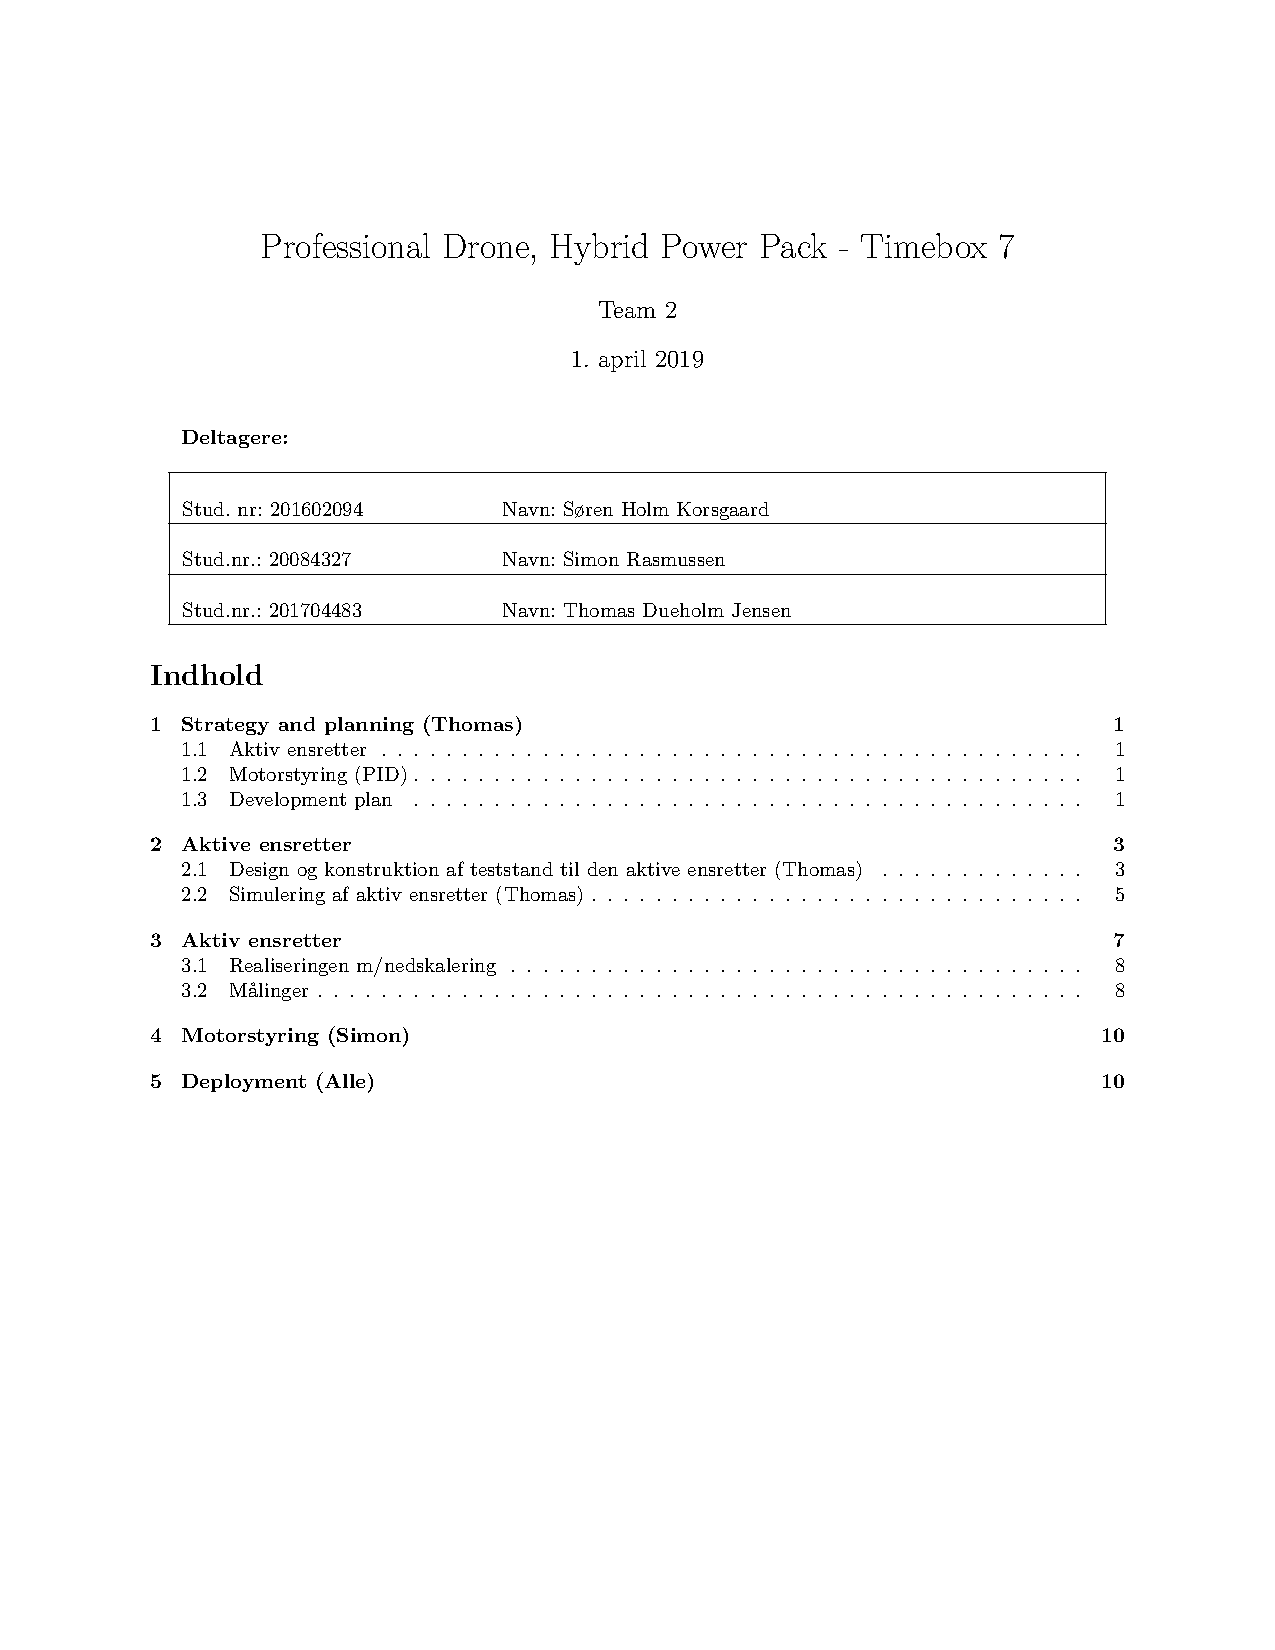
\includepdf[pages={-1}]{timebox7}
\clearpage

\addcontentsline{toc}{section}{Timebox 8}
\label{sec:timebox-8}
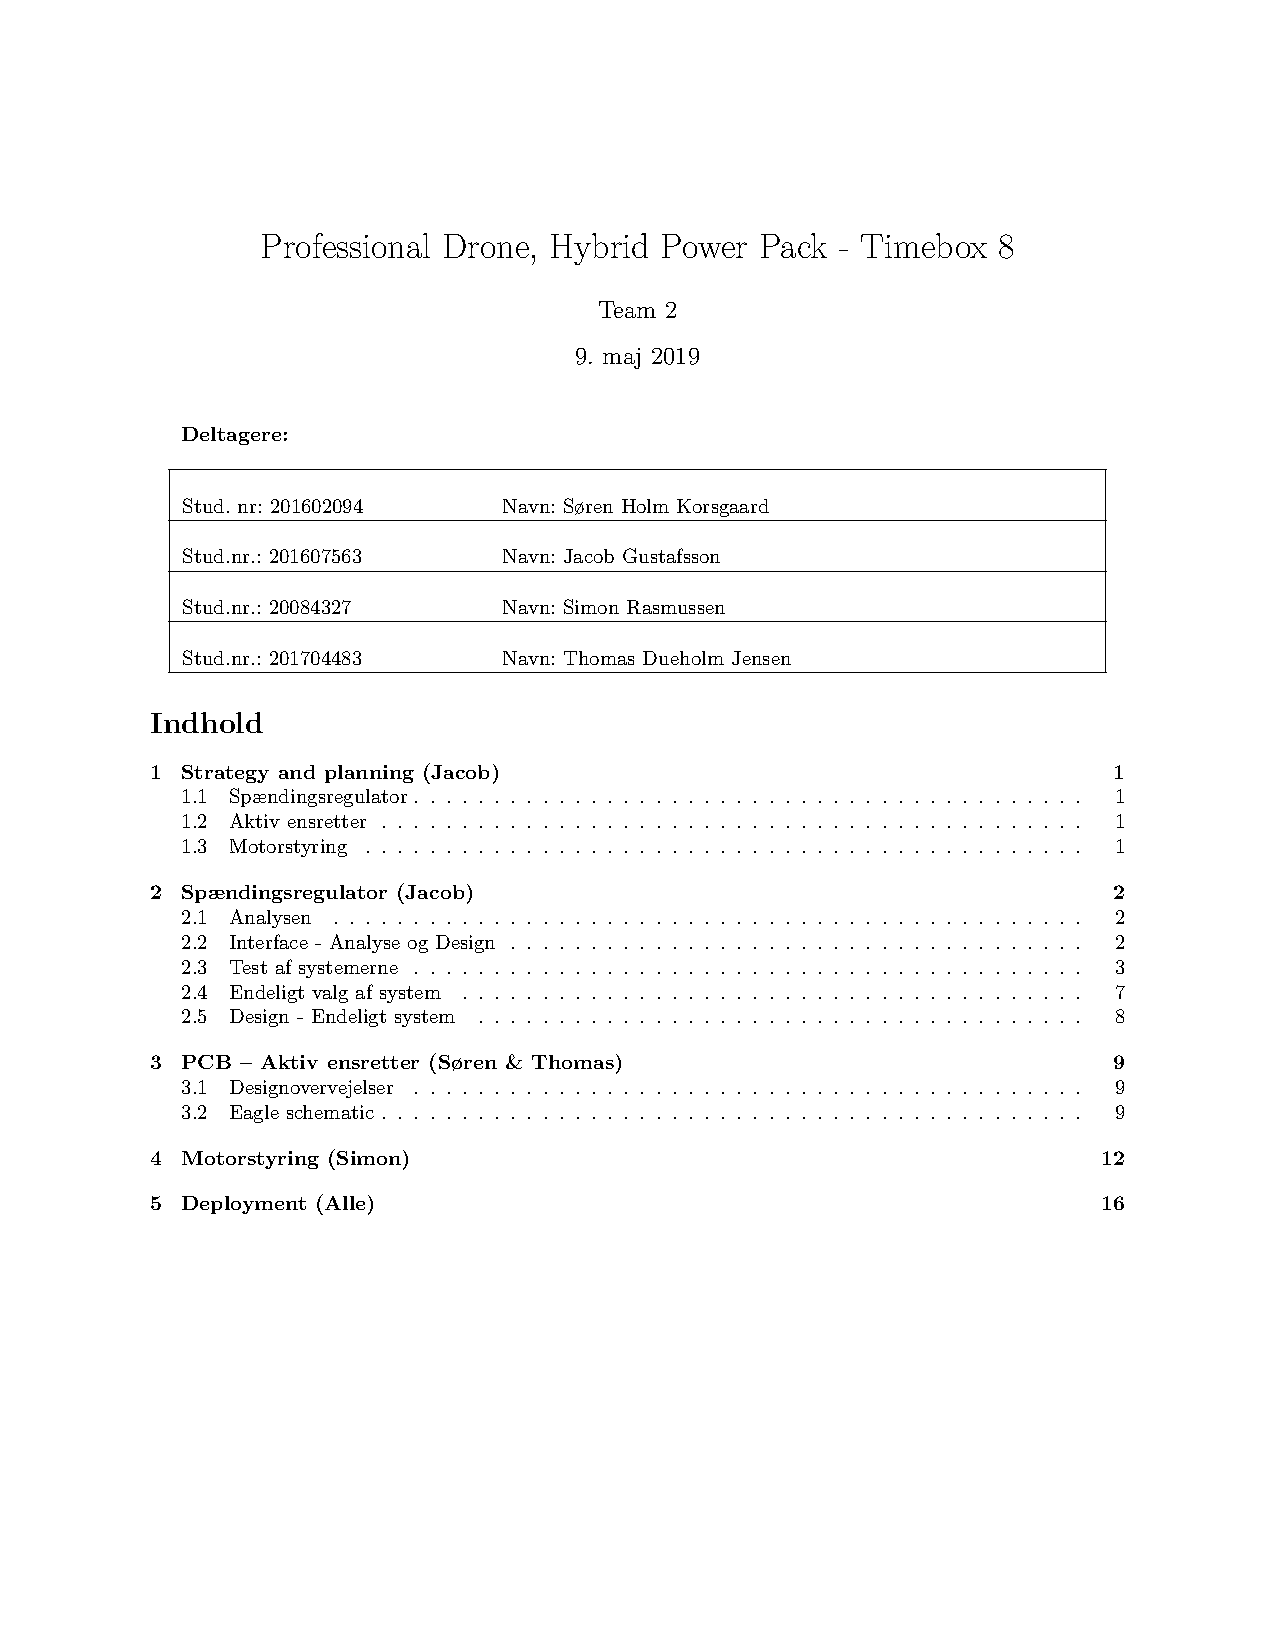
\includepdf[pages={-1}]{timebox8}
\clearpage

\addcontentsline{toc}{section}{Timebox 9}
\label{sec:timebox-9}
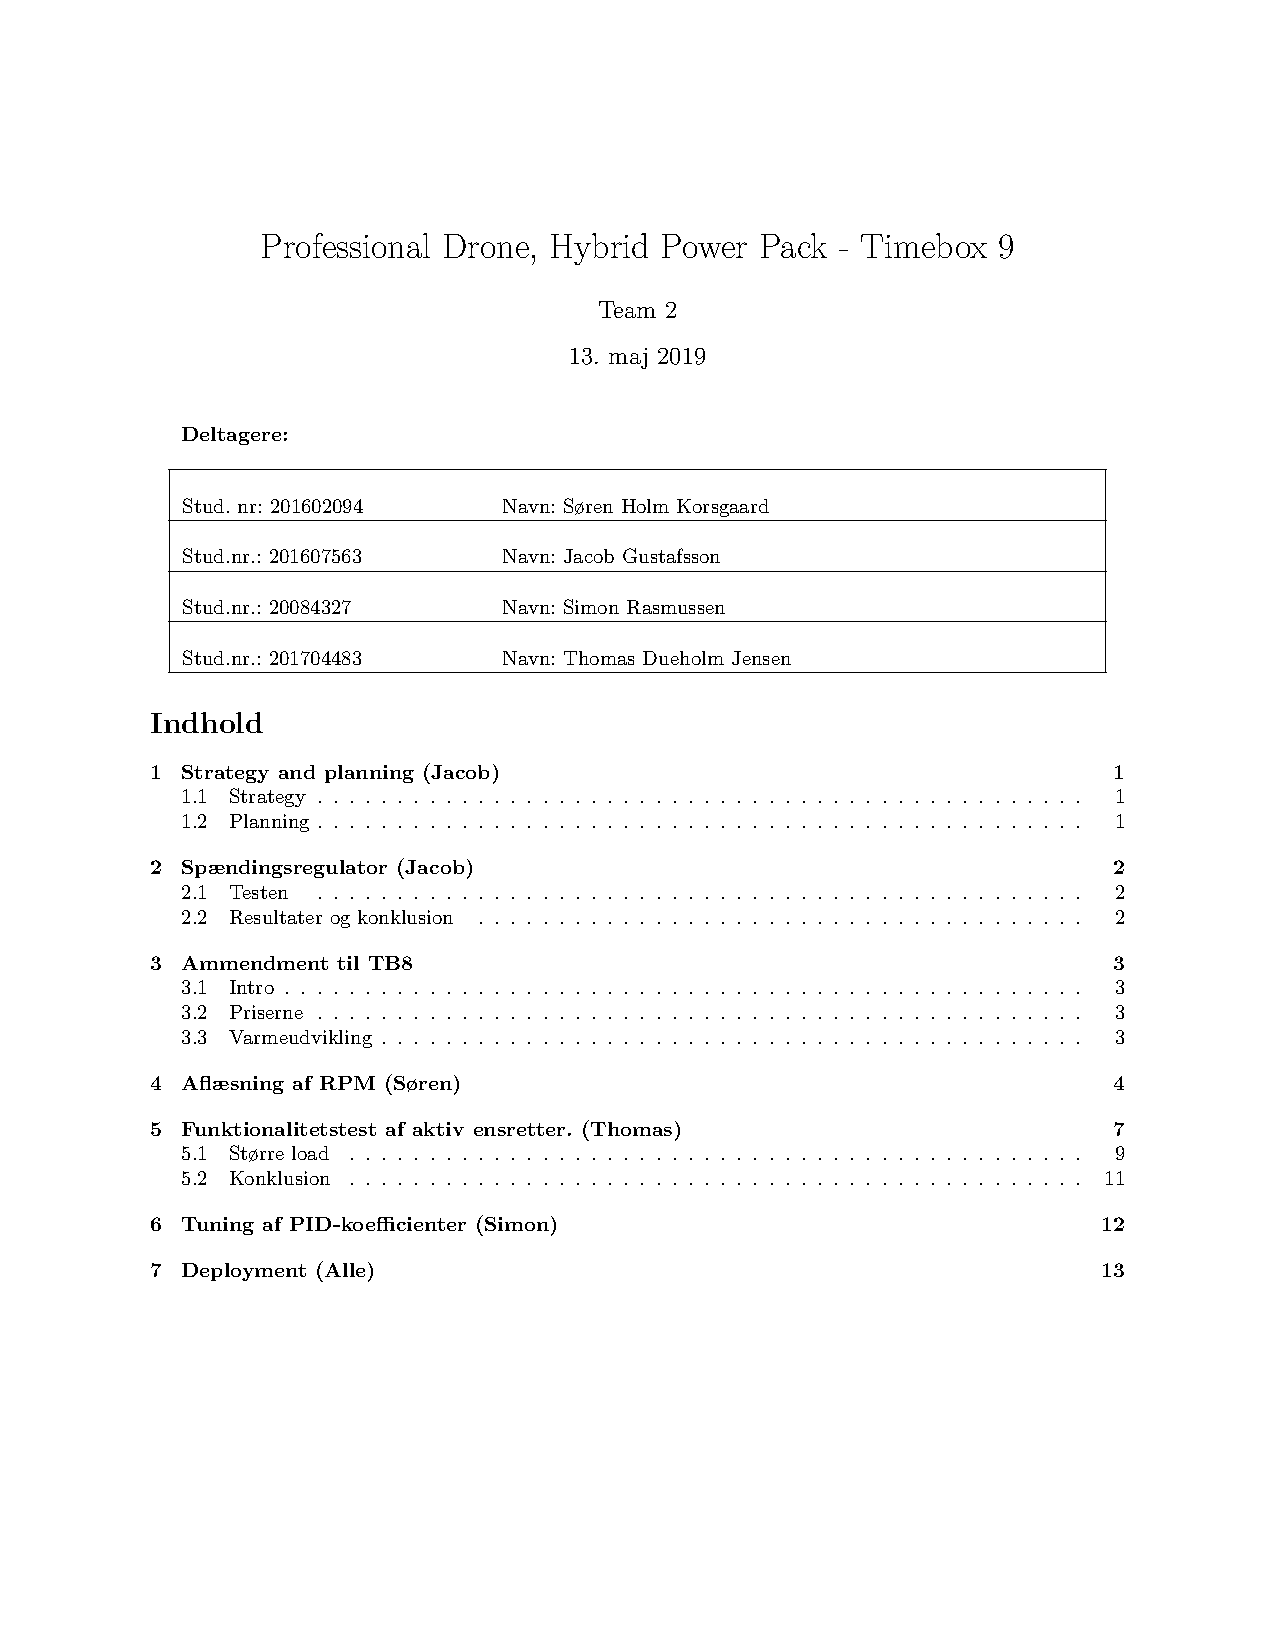
\includepdf[pages={-1}]{timebox9}
\clearpage

\end{document}